\section{Event Selection and Analysis \label{sec:selection}}

The analysis follows closely Ref.~\cite{RA1Paper}.  Events with two or
more high-\pt jets, reconstructed using the anti-k$_\text{T}$
algorithm~\cite{antikt} with a size parameter of $0.5$ are
selected. Jets are required to have $\Et>50\gev$, $|\eta| < 3$ and to
pass jet identification criteria~\cite{JME-09-008} designed to reject
spurious signals and noise in the calorimeters. The pseudorapidity of
the jet with the highest \Et~(leading jet) is required to be within
$|\eta|<2.5$, and the transverse energy of each of the two leading
jets must exceed 100\gev.

Events with jets passing the \Et\ threshold but not satisfying the jet
identification criteria or the $\eta$ acceptance requirement are
vetoed, as this deposited energy is not accounted for in the event
kinematics. Similarly, events in which an isolated lepton (electron or
muon) with $\pt > 10\gev$ is identified are rejected to suppress
events with genuine missing energy from neutrinos.  The electron and
muon selection requirements are described in ~\cite{PAS-EGM-10-004}
and~\cite{PAS-MUO-10-002}, respectively.  Furthermore, to select a
pure multi-jet topology, events are vetoed in which an isolated
photon~\cite{PAS-EGM-10-005} with $\pt > 25\gev$ is found.

Events are required to satisfy $\HT > 275 \gev$.  As the main
discriminator against QCD multijet production the variable \alt,
defined for di-jet events as:

\begin{equation*}
\label{eq:alt}
\alt = \frac{\Et^{\rm jet_2}}{M_\text{T}} =  \frac{\Et^{\rm jet_2}}{\sqrt{ \left( \sum_{i=1}^2
\Et^{{\rm jet}_i} \right)^2 - \left( \sum_{i=1}^2 p_x^{{\rm jet}_i} \right)^2 - \left(
\sum_{i=1}^2 p_y^{{\rm jet}_i} \right)^2}},
\end{equation*}

is used and events are required to have $\alt > 0.55$.
In events with jet multiplicity $n > 2$, two pseudo-jets are formed
following Ref.~\cite{RA1Paper} and Eq.~\ref{eq:alt} is applied to the
pseudo-jets.

To protect against multiple jets failing the $\Et>50\gev$ selection
requirement, the jet-based estimate of the missing transverse energy,
\mht, is compared to the calorimeter tower-based estimate, $\met^{\rm
  calo}$, and events with $R_{\rm miss}=\mht/\met^{\rm calo} > 1.25$
are rejected.

Finally, to protect against severe energy losses, events with
significant jet mismeasurements caused by masked regions in the ECAL
(which amount to about 1\% of the ECAL channel count), or by missing
instrumentation in the barrel-endcap gap, are removed with the
following procedure. The jet-based estimate of the missing transverse
energy, \mht, is used to identify jets most likely to have given rise
to the \mht as those whose momentum is closest in $\phi$ to the total
$\vec{\mht}$ which results after removing them from the event.  The
azimuthal distance between this jet and the recomputed \mht is
referred to as $\Delta\phi^*$ in what follows. Events with
$\Delta\phi^* < 0.5$ are rejected if the distance in the ($\eta,\phi$)
plane between the selected jet and the closest masked ECAL region,
$\Delta R_{\rm ECAL}$, is smaller than 0.3. Similarly, events are
rejected if the jet points within 0.3 in $\eta$ of the ECAL
barrel-endcap gap at $|\eta| = 1.5$.

To increase the sensitivity to higher-mass states, we carry out a
shape analysis over the entire $\HT > 275 \gev$ region.  This requires
that the Standard Model background estimation methods which are based
on data control samples, provide an estimate of the background for
each of the \scalht bins in the signal region with $\scalht > 275
\gev$. The background estimation methods based on data control samples
as used in Ref.~\cite{RA1Paper} were explicitly designed with this
use-case in mind.  In the following, the results for the different
background prediction methods are presented when splitting the signal
region into 8 bins, as defined in Table~\ref{tab:results-HT}.

The results of this selection are documented in
Table~\ref{tab:results-HT} and comparisons between Data and Monte
Carlo (MC) simulation for control variables are shown in
Section~\ref{sub:data_to_monte_carlo_comaprison_for_control_variables}.

\begin{table}[ht!]
\caption{Definition of the \HT bins and the corresponding \pt
  thresholds for the leading, second, and all remaining  jets
  in the event; the number of events passing and failing the \alt cut
  and the resulting \RaT value, for 1.1 fb$^{-1}$ of data
  collected in 2011.}
\label{tab:results-HT}
\centering
\footnotesize
\begin{tabular}{ c|c|c|c|c }

\hline
\scalht Bin (GeV)       & 275--325                       & 325--375                       & 375--475                       & 475--575                       \\ [0.5ex]
$\pt^{\rm leading}$ (GeV) & 73 & 87 & 100 & 100 \\
$\pt^{\rm second}$ (GeV) & 73 & 87 & 100 & 100 \\
$\pt^{\rm other}$(GeV) & 37 & 43 & 50 & 50 \\  
\hline
$\alt > 0.55$           & 782                            & 321                            & 196                            & 62                             \\ 
$\alt < 0.55$           & 5.73 $\cdot 10^7$                       & 2.36 $\cdot 10^7$                       & 1.62 $\cdot 10^7$                      & 5.12 $\cdot 10^6$\\ 
$\RaT (10^{-5})$       & $ 1.36 \pm 0.05_{\rm stat}$ & $1.36 \pm 0.08_{\rm stat}$ & $1.21 \pm 0.09_{\rm  stat}$ & $1.21 \pm 0.15_{\rm stat}$ \\ 

\hline
\scalht Bin (GeV)       & 575--675                       & 675--775                       & 775--875                       & 875--$\infty$                  \\ [0.5ex]
$\pt^{\rm leading}$ (GeV) & 100 & 100 & 100 & 100 \\
$\pt^{\rm second}$ (GeV) & 100 & 100 & 100 & 100 \\
$\pt^{\rm other}$ (GeV) & 50 & 50 & 50 & 50 \\

\hline
$\alt > 0.55$           & 21                             & 6                              & 3                              & 1                              \\ 
$\alt < 0.55$           & 1.78 $\cdot 10^6$                       &6.89 $\cdot 10^5$                      & 2.90 $\cdot 10^5$                       & 2.60 $\cdot 10^5$\\ 
$\RaT (10^{-5})$       & $1.18 \pm 0.26_{\rm stat}$ & $0.87 \pm 0.36_{\rm stat}$ & $1.03 \pm 0.60_{\rm stat}$ & $0.39 \pm 0.52_{\rm stat}$ \\ 

\hline
\end{tabular}
\end{table}

\subsection{Data to Monte Carlo Comparison for Analysis Variables} % (fold)
\label{sub:data_to_monte_carlo_comaprison_for_control_variables}

In the following we show data--MC comparisons before the $\alt > 0.55$
selection and requiring $\HT > 375 \gev$ and $\mht > 100 \gev$,
slightly higher than the trigger requirement.  The data--MC comparison
plots are used to demonstrate the quality of the simulation, but are
not used for the background prediction.  The actual background yields
are obtained from data control samples, as described further below.
The uncertainties displayed on the MC distributions only correspond to
the statistical uncertainties and do not include systematic
uncertainties due to, e.g., jet energy scale or resolution.

\begin{figure}[h!]
    \centering
     \subfigure[Comparison of \HT between data and MC for the
     hadronic selection for \HT $\geq$ 375 \GeV and $\mht > 100 \gev$. 
]{
          \label{fig:figures_HT_all}
          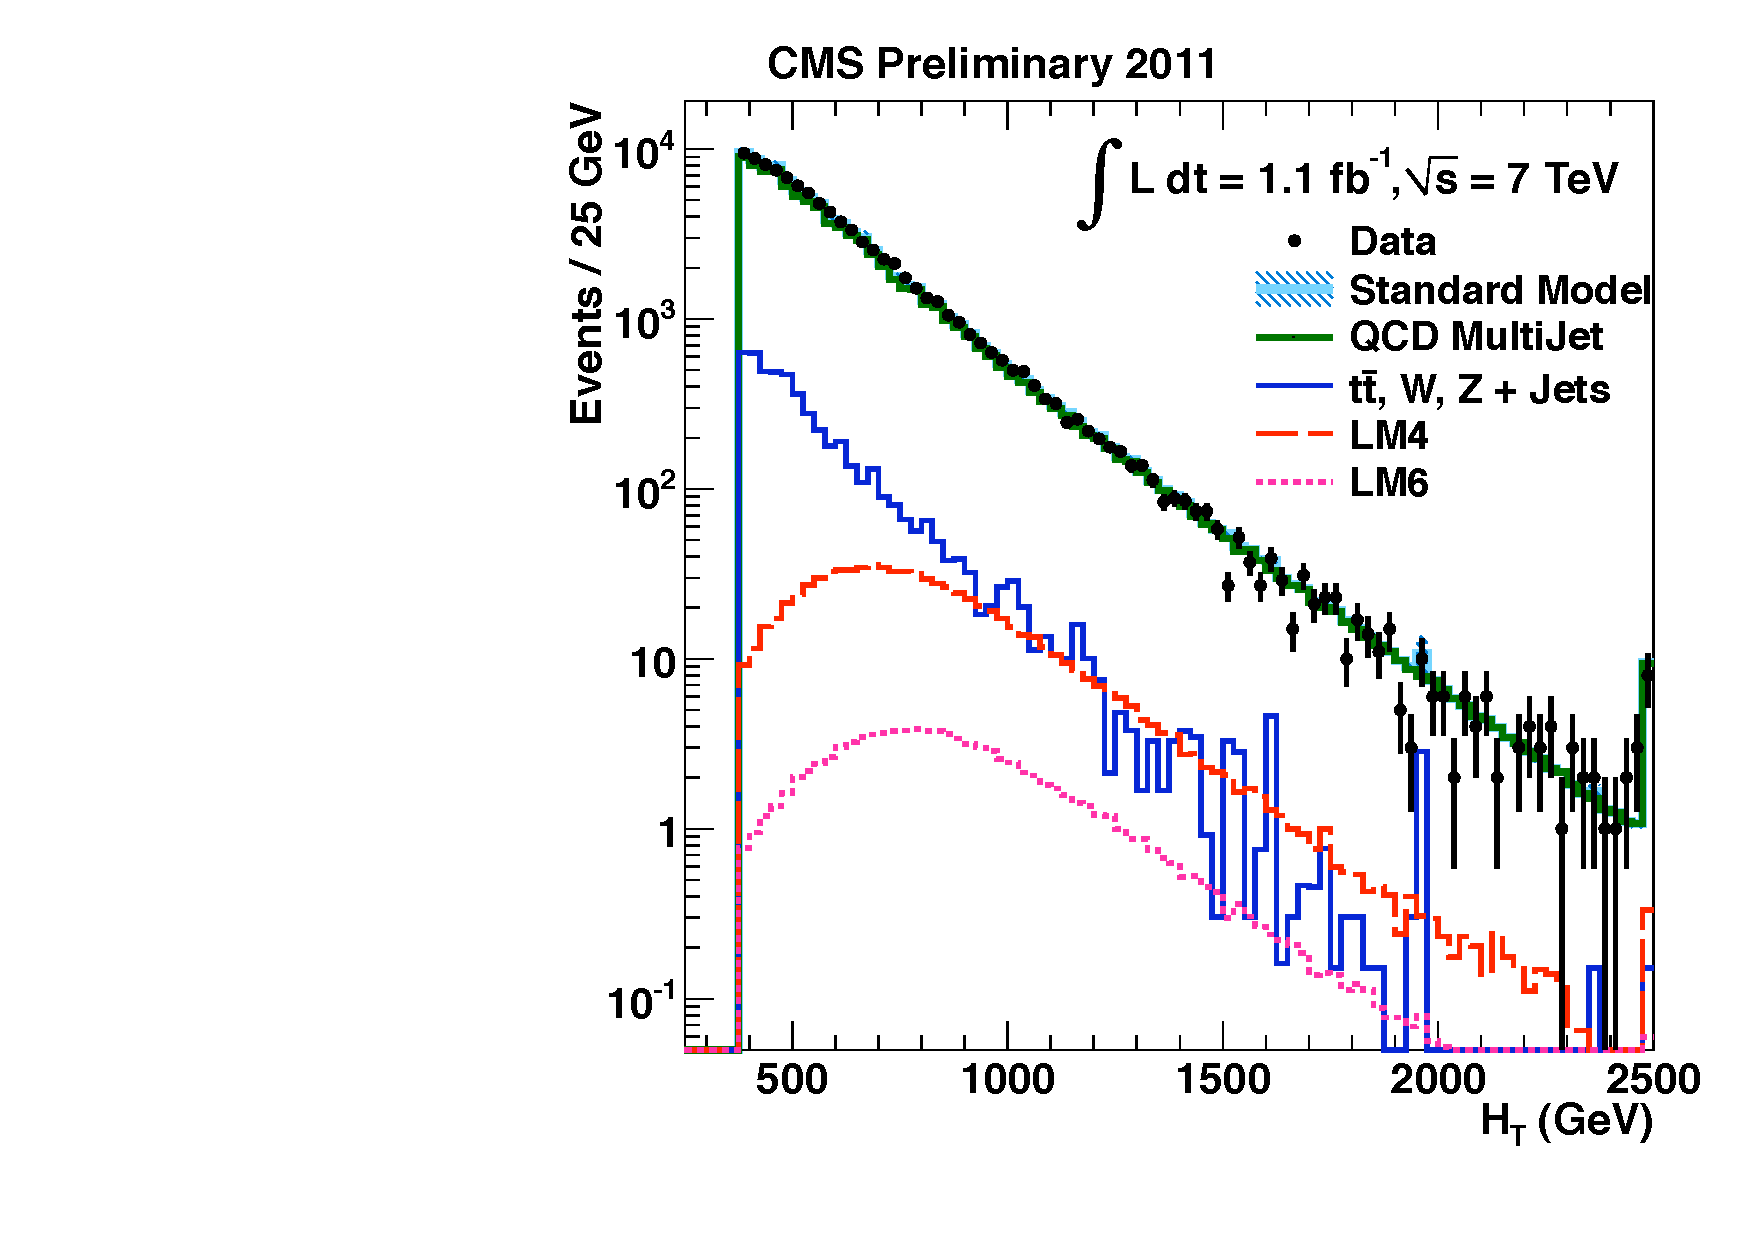
\includegraphics[width=0.46\textwidth]{figures/HT_all.pdf}
     }
\hspace{0.3cm}
    \subfigure[Comparison of the jet multiplicity between data and
    MC for the hadronic selection, for \HT $\geq$ 375 \GeV
    and $\mht > 100 \gev$.
]{
          \label{fig:figures_JetMultiplicity_all}
          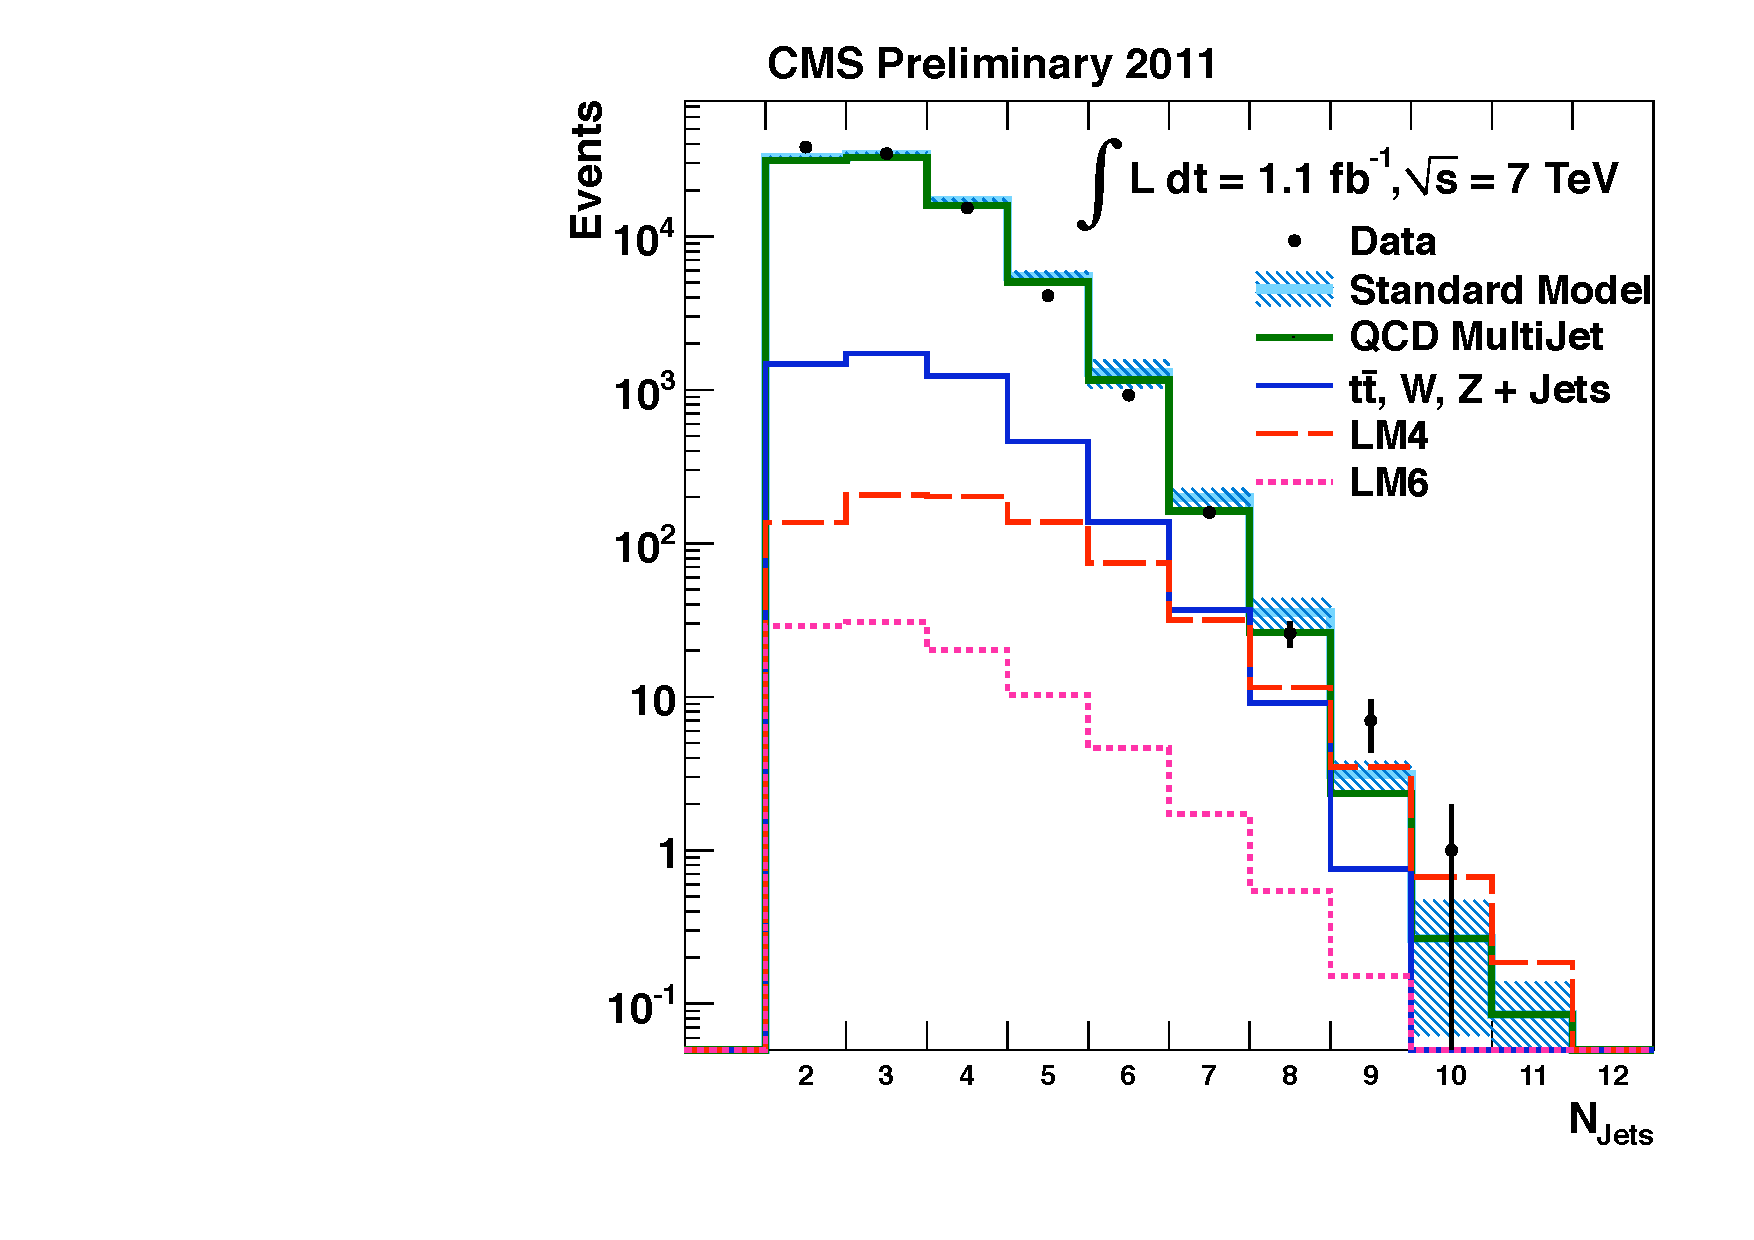
\includegraphics[width=0.46\textwidth]{figures/JetMultiplicity_all.pdf}
     }
    \newline
    \subfigure[Comparison of the \alt distribution between data and
    MC for the hadronic selection, for \HT $\geq$ 375 \GeV
    and $\mht > 100 \gev$.
]{
          \label{fig:figures_AlphaT_all}
          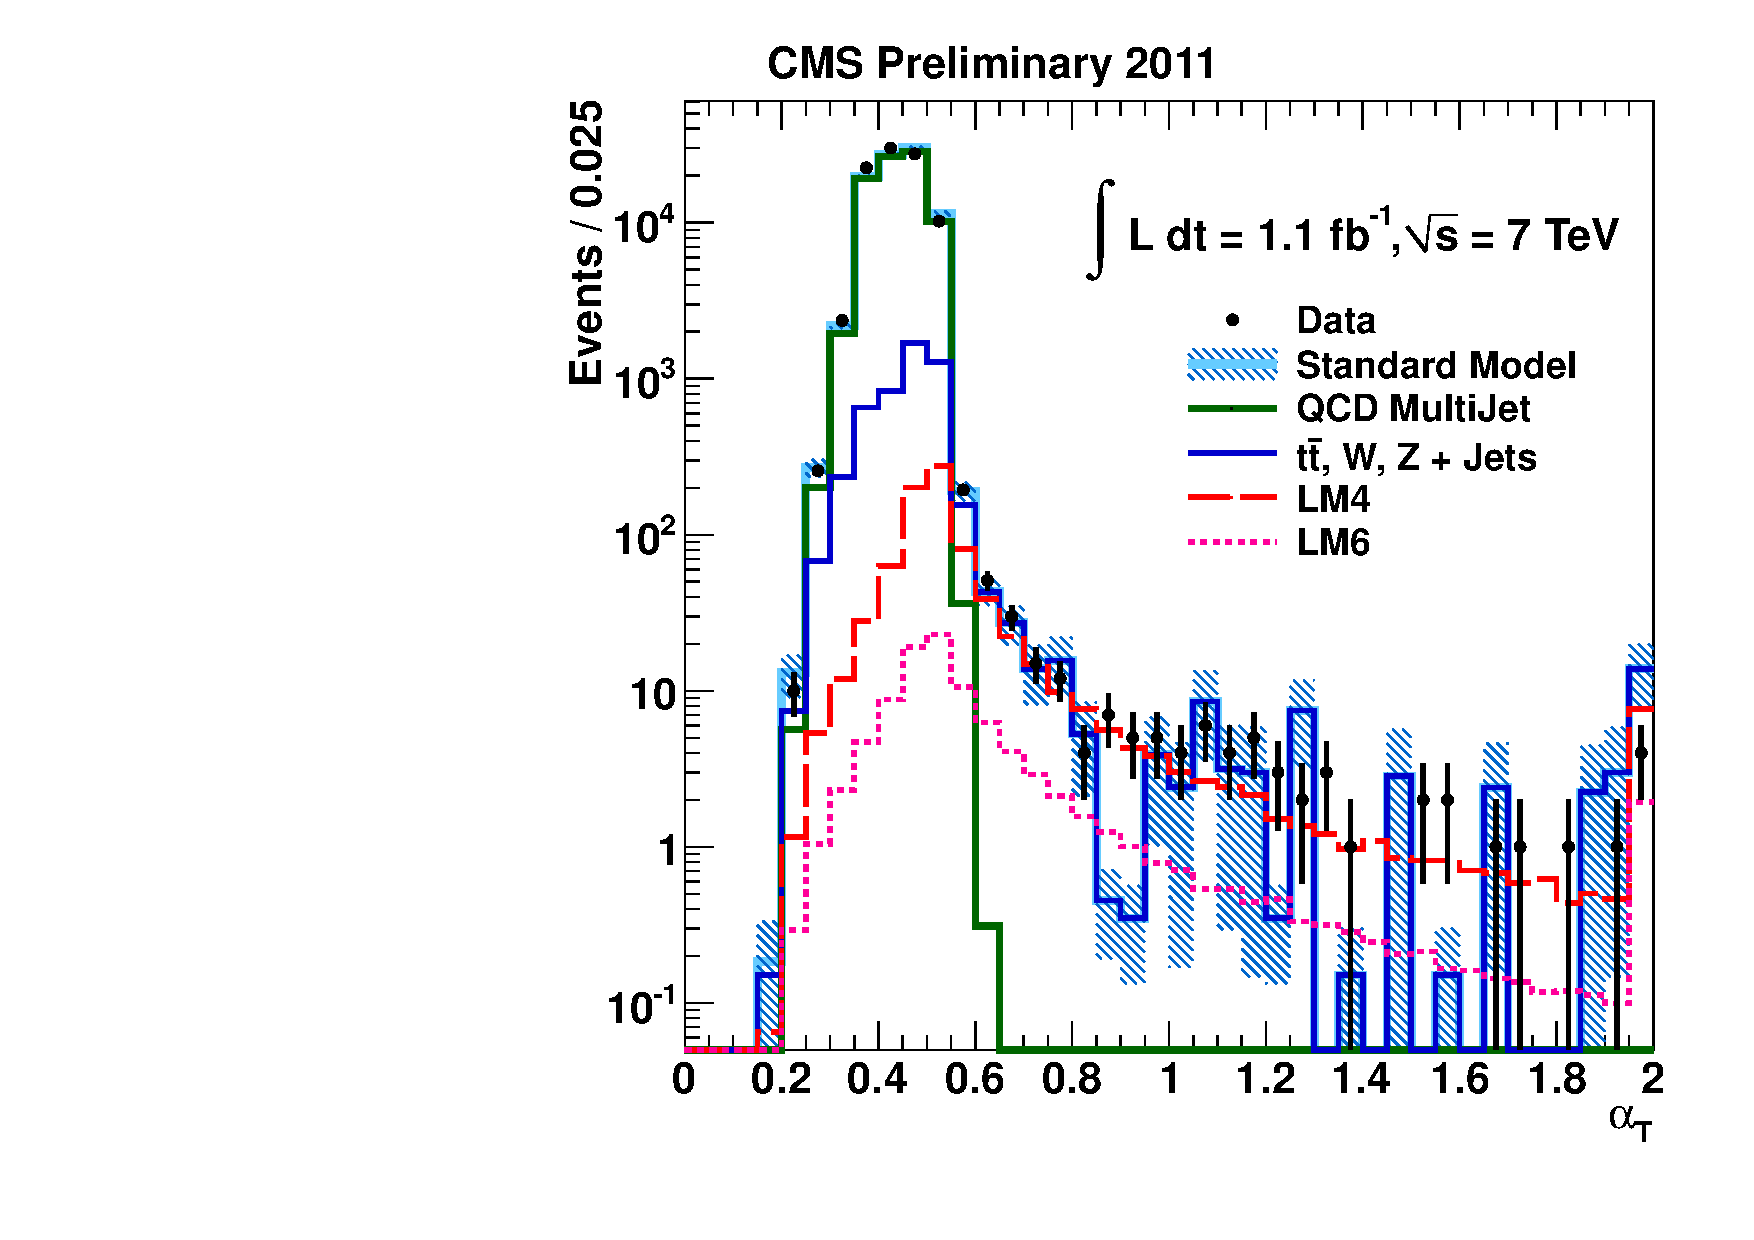
\includegraphics[width=0.46\textwidth]{figures/AlphaT_all.pdf}
     }
 %   \subfigure[Comparison of the \alt distribution highlighting the agreement on the sharply falling edge between Data and Monte Carlo for the hadronic selection, in the region \HT $\geq$ 375 \GeV.]{
%          \label{fig:figures_AlphaT_Zoomed_all}
%          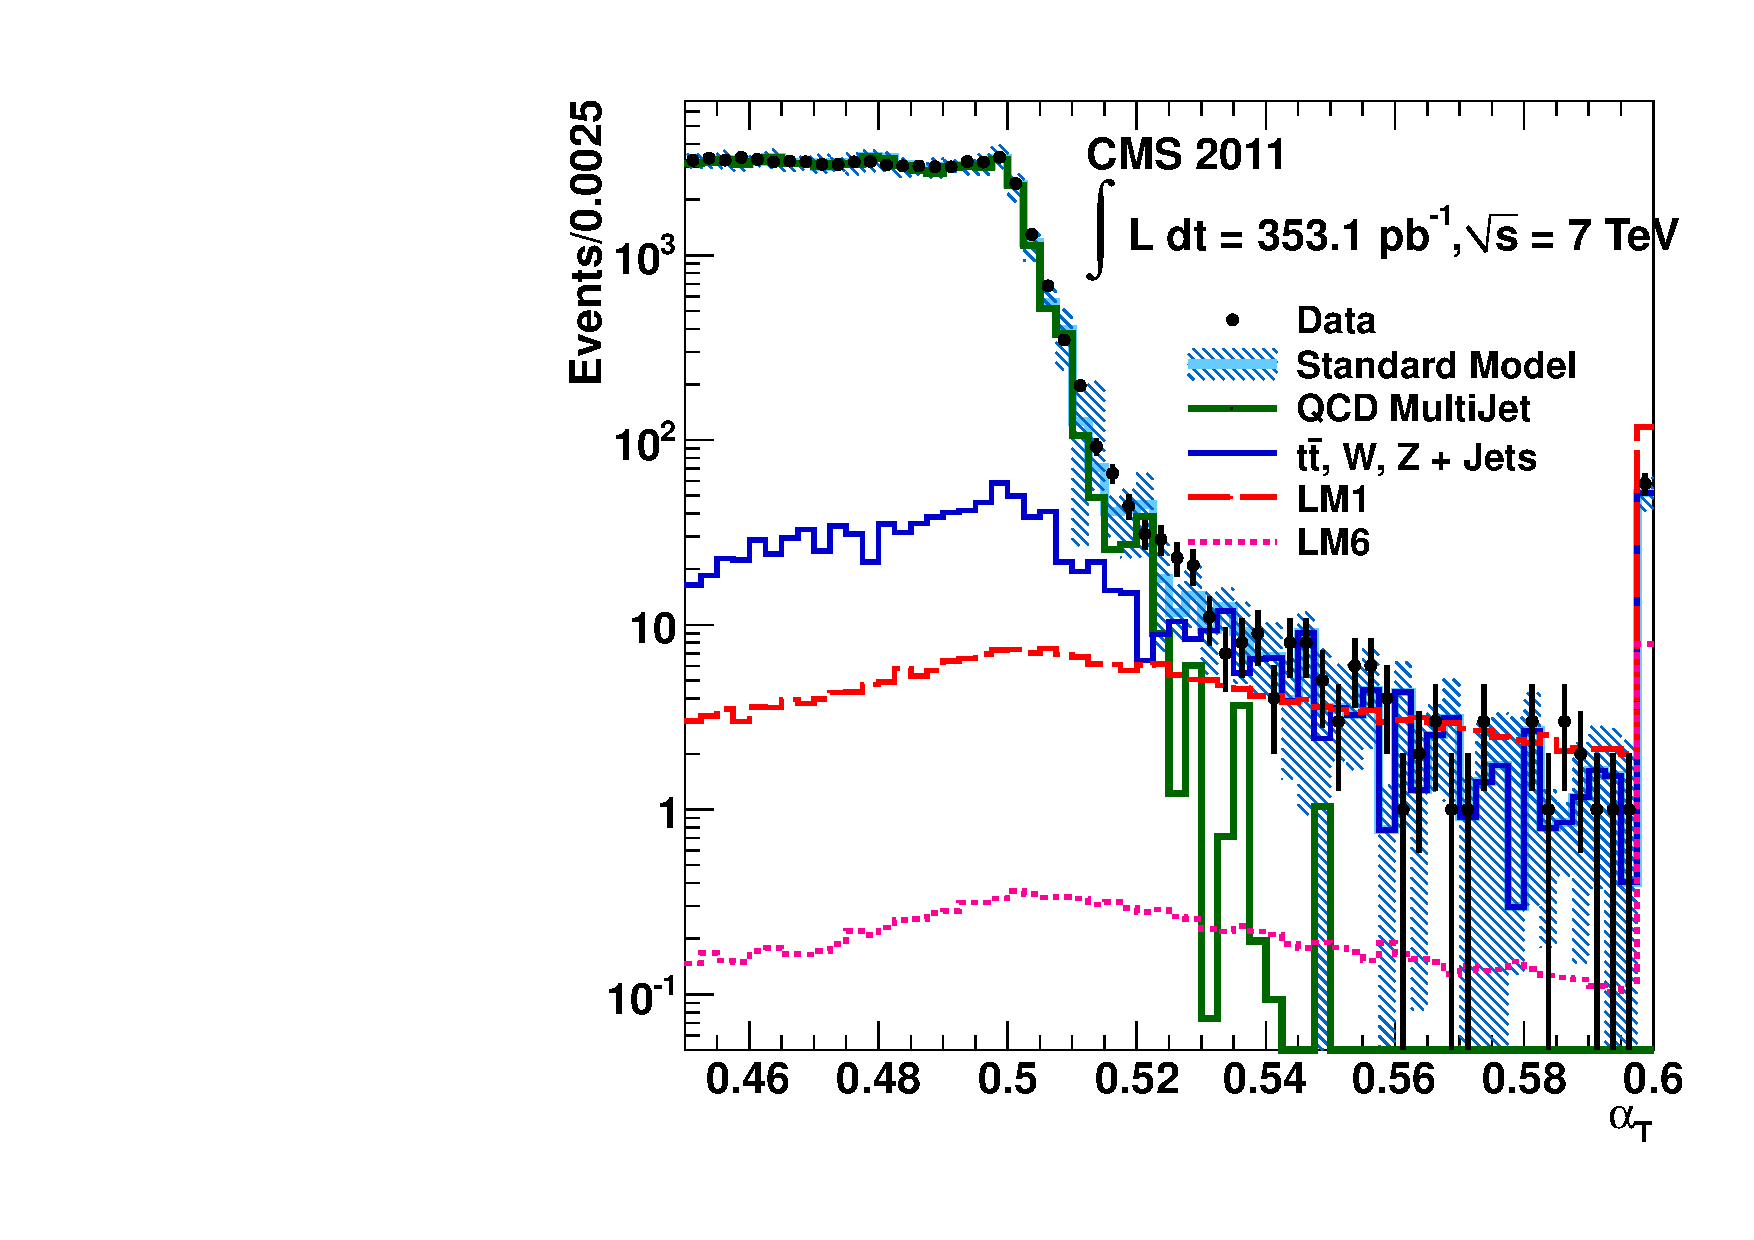
\includegraphics[width=0.46\textwidth]{figures/AlphaT_Zoomed_all.pdf}
     }
    \caption{Comparisons of basic quantities before the \alt selection cuts.}
\end{figure}

Figures~\ref{fig:figures_HT_all}
and~\ref{fig:figures_JetMultiplicity_all} show the comparisons between
data and MC simulation for the \HT variable and the number of
reconstructed jets per event, before the requirement on \alt. Good
agreement is observed between data and MC simulation.

Figure~\ref{fig:figures_AlphaT_all} shows the \alt distribution and
demonstrates that this variable is an excellent discriminator between
QCD background and signal.  The number of expected QCD events quickly
falls to zero with increasing \alt.


\begin{figure}[h!]
    \centering
     \subfigure[$\Delta \Phi^{*}$ distribution after \alt selection.]{
          \label{fig:BiasedDeltaPhi_after_alphaT_55_all}
          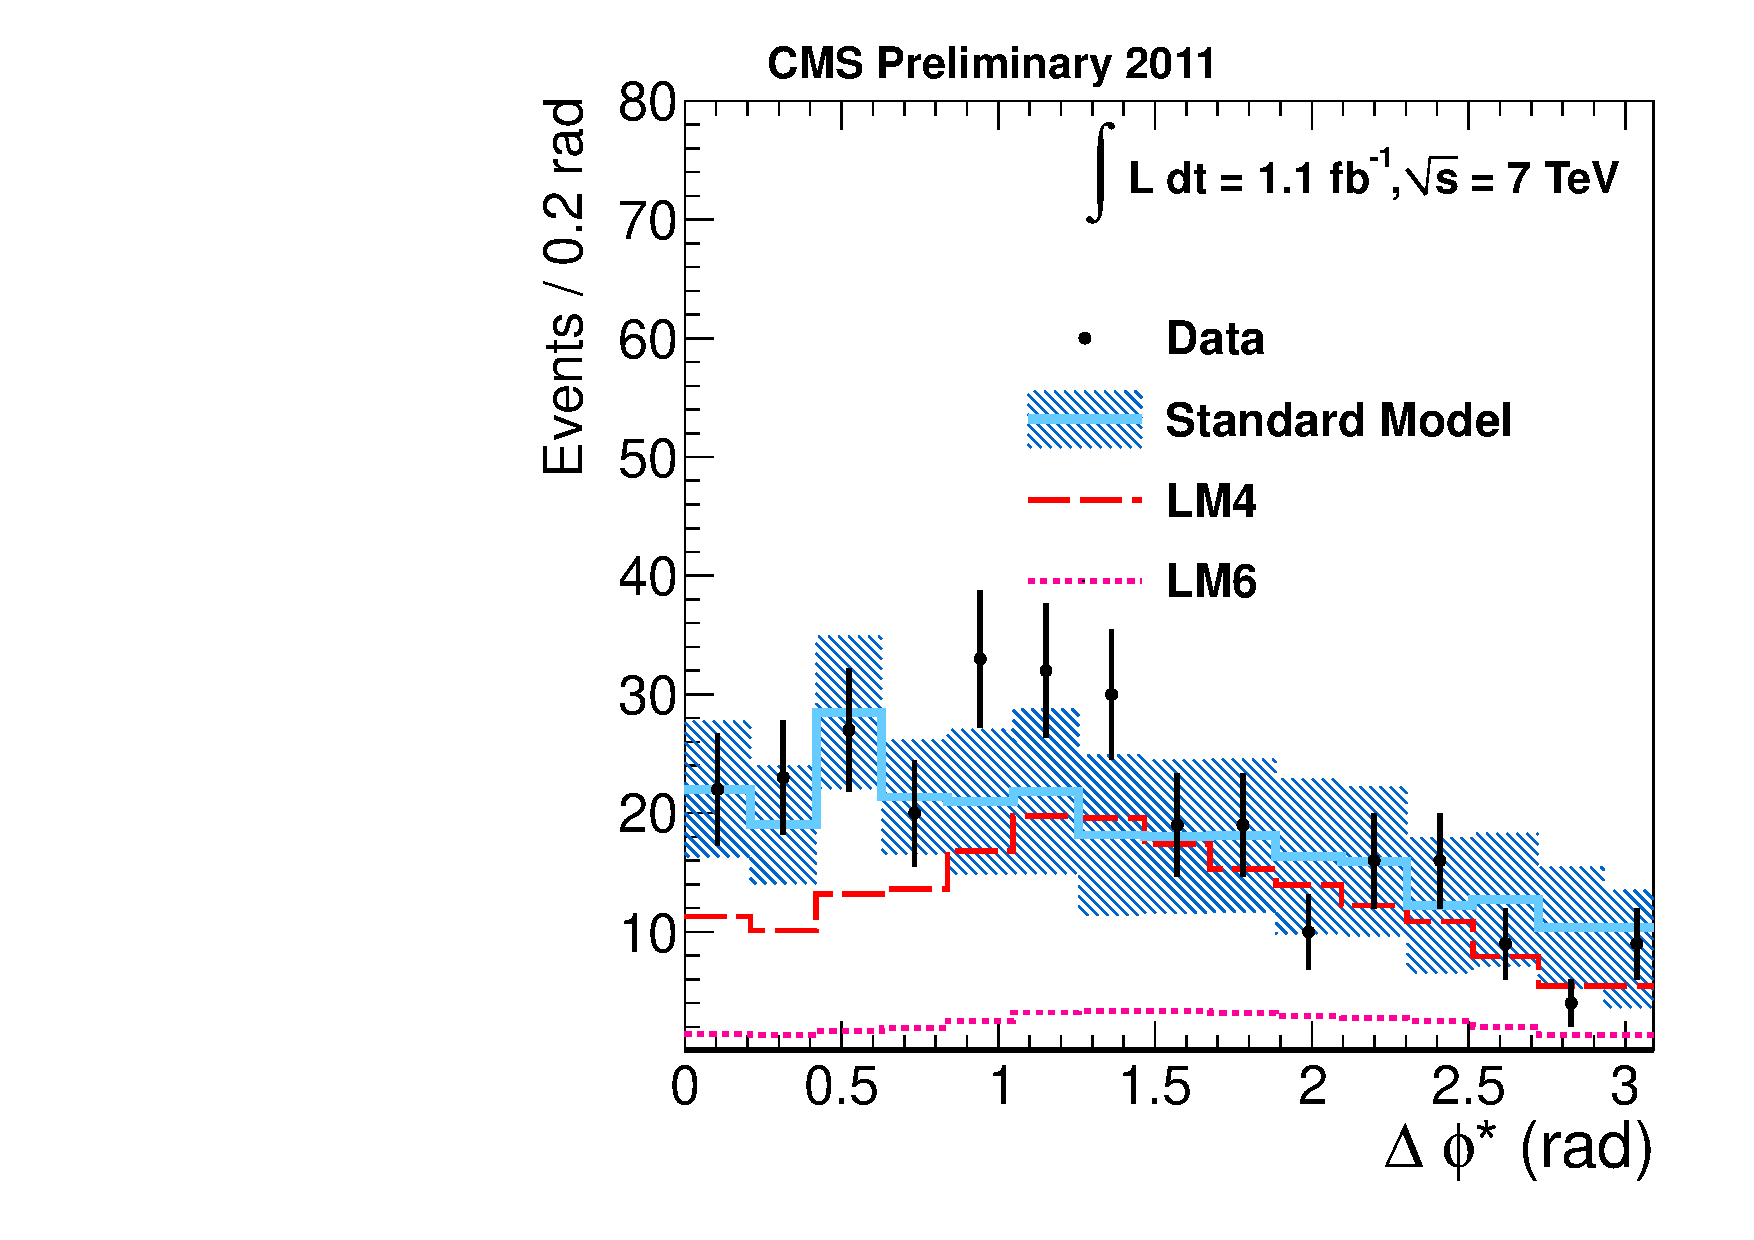
\includegraphics[width=0.46\textwidth]{figures/BiasedDeltaPhi_after_alphaT_55_all.pdf}
     }
\hspace{0.3cm}
    \subfigure[The effective mass distribution, $M_{\rm eff} = \HT +
    \mht$, of the events passing the \alt selection.]{
          \label{fig:EffectiveMass_after_alphaT_55_all}
          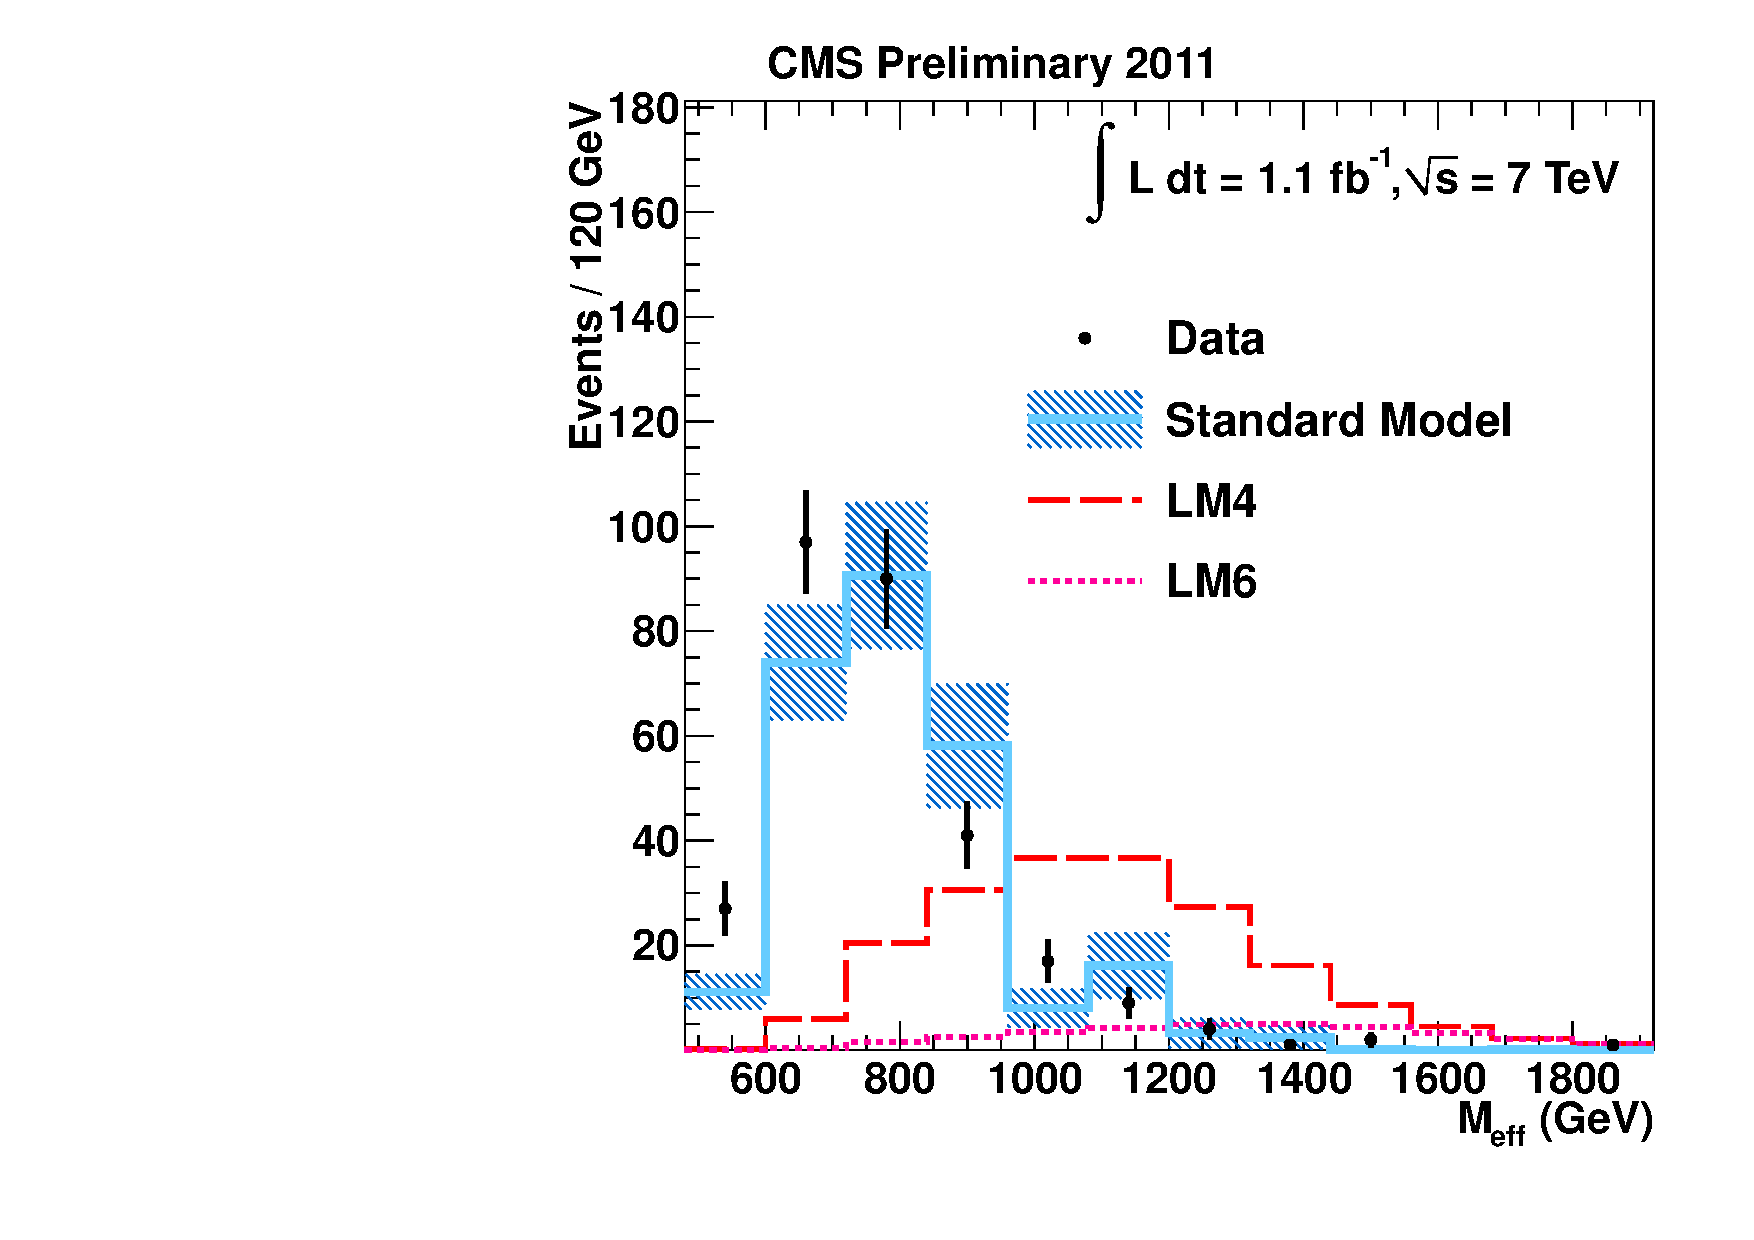
\includegraphics[width=0.46\textwidth]{figures/EffectiveMass_after_alphaT_55_all.pdf}
     }
    \newline
    \subfigure[Jet multiplicity after \alt selection.]{
          \label{fig:JetMultiplicityAfterAlphaT_all}
          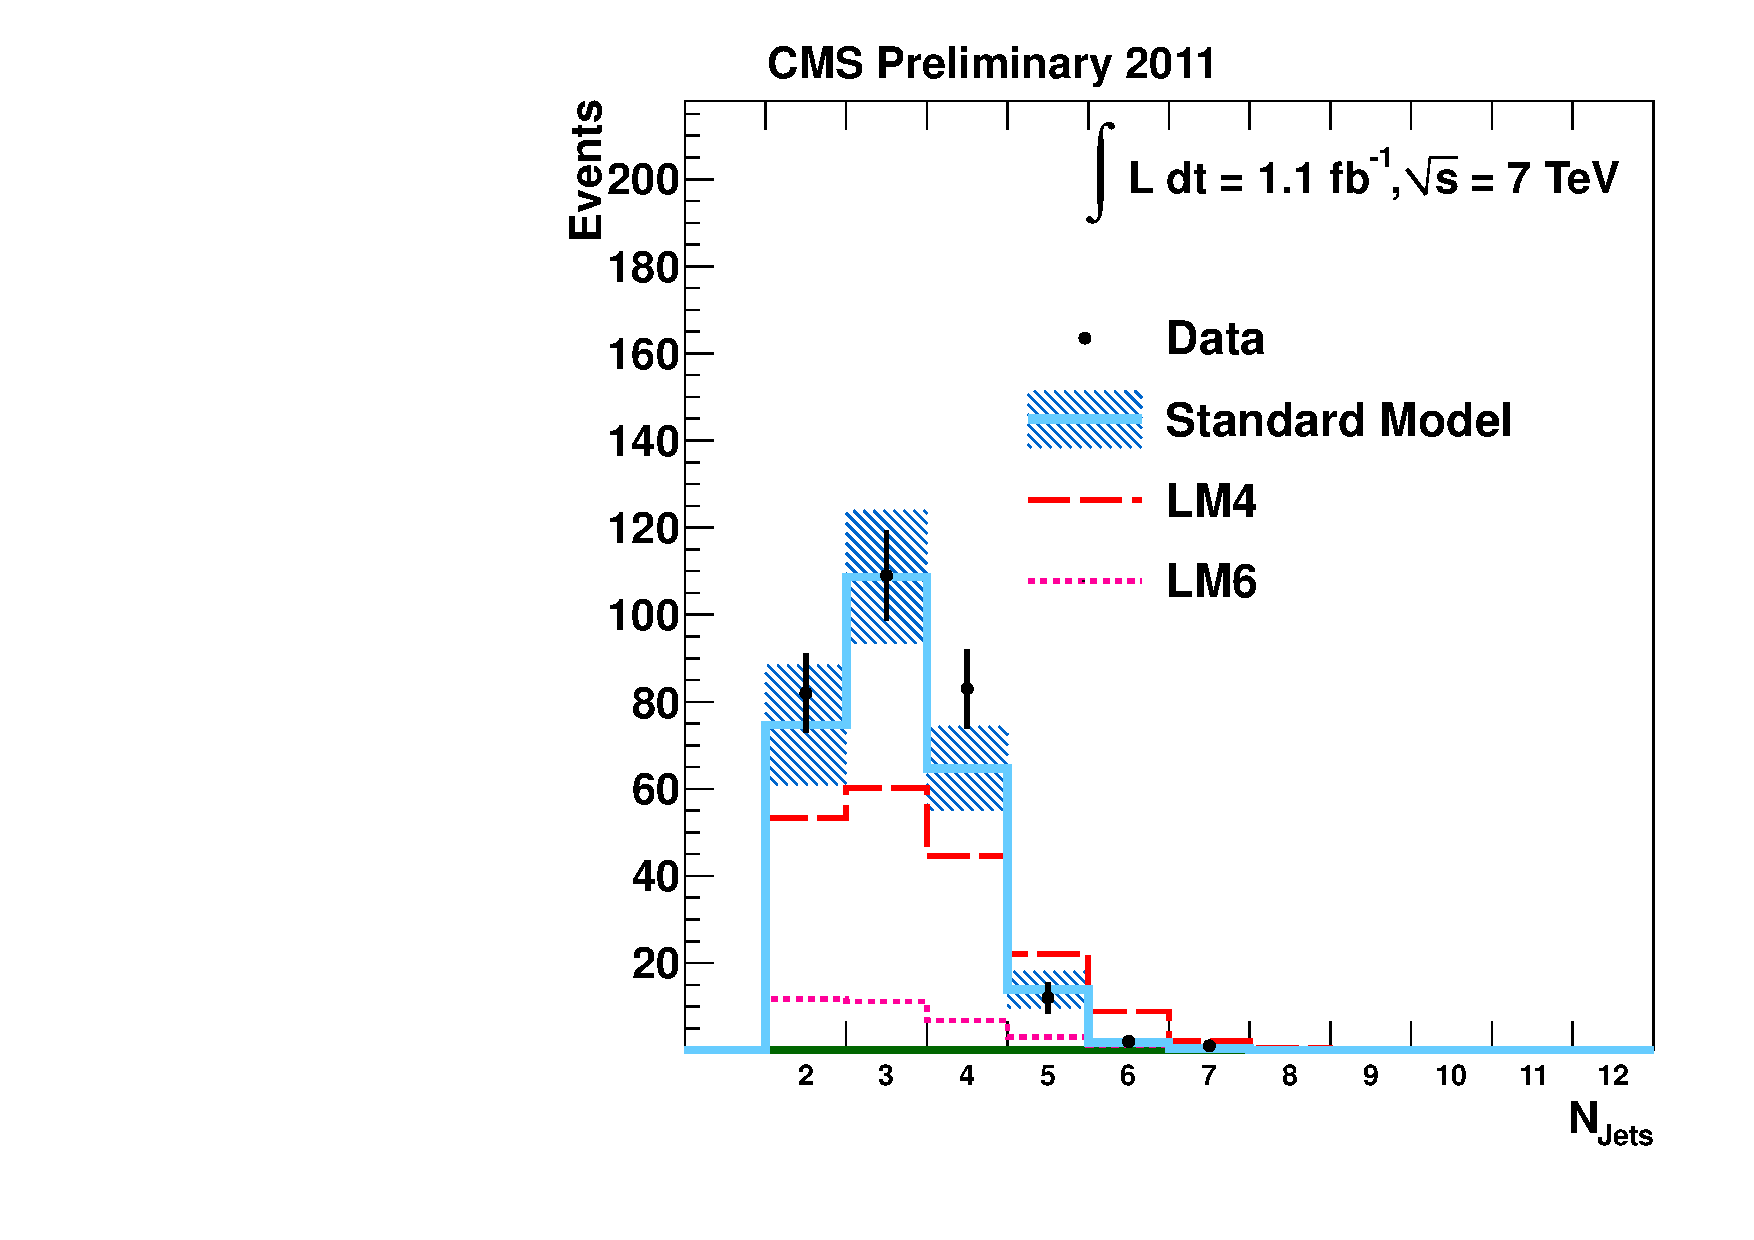
\includegraphics[width=0.46\textwidth]{figures/JetMultiplicityAfterAlphaT_all.pdf}
     }
\caption{Comparisons between data and MC after the \alt selection cut.}
\end{figure}

Figures~\ref{fig:BiasedDeltaPhi_after_alphaT_55_all},
\ref{fig:EffectiveMass_after_alphaT_55_all}
and~\ref{fig:JetMultiplicityAfterAlphaT_all} show comparisons between
simulated standard model distributions and data for events passing the
\alt selection.  The $\Delta\phi^*$ distribution in
Figure~\ref{fig:BiasedDeltaPhi_after_alphaT_55_all} shows an
approximately flat behaviour as expected from SM processes with real
missing transverse energy such as \ttbar, W + jets and \znunu +jets
events. No evidence for QCD multi-jet events which would peak at small
values of $\Delta\phi^*$ is seen.  Generally, the observed
distributions in data show no deviation from the standard model
prediction.

% subsection data_to_monte_carlo_comaprison_for_control_variables (end)

\begin{figure}[!h]
  \begin{center}
    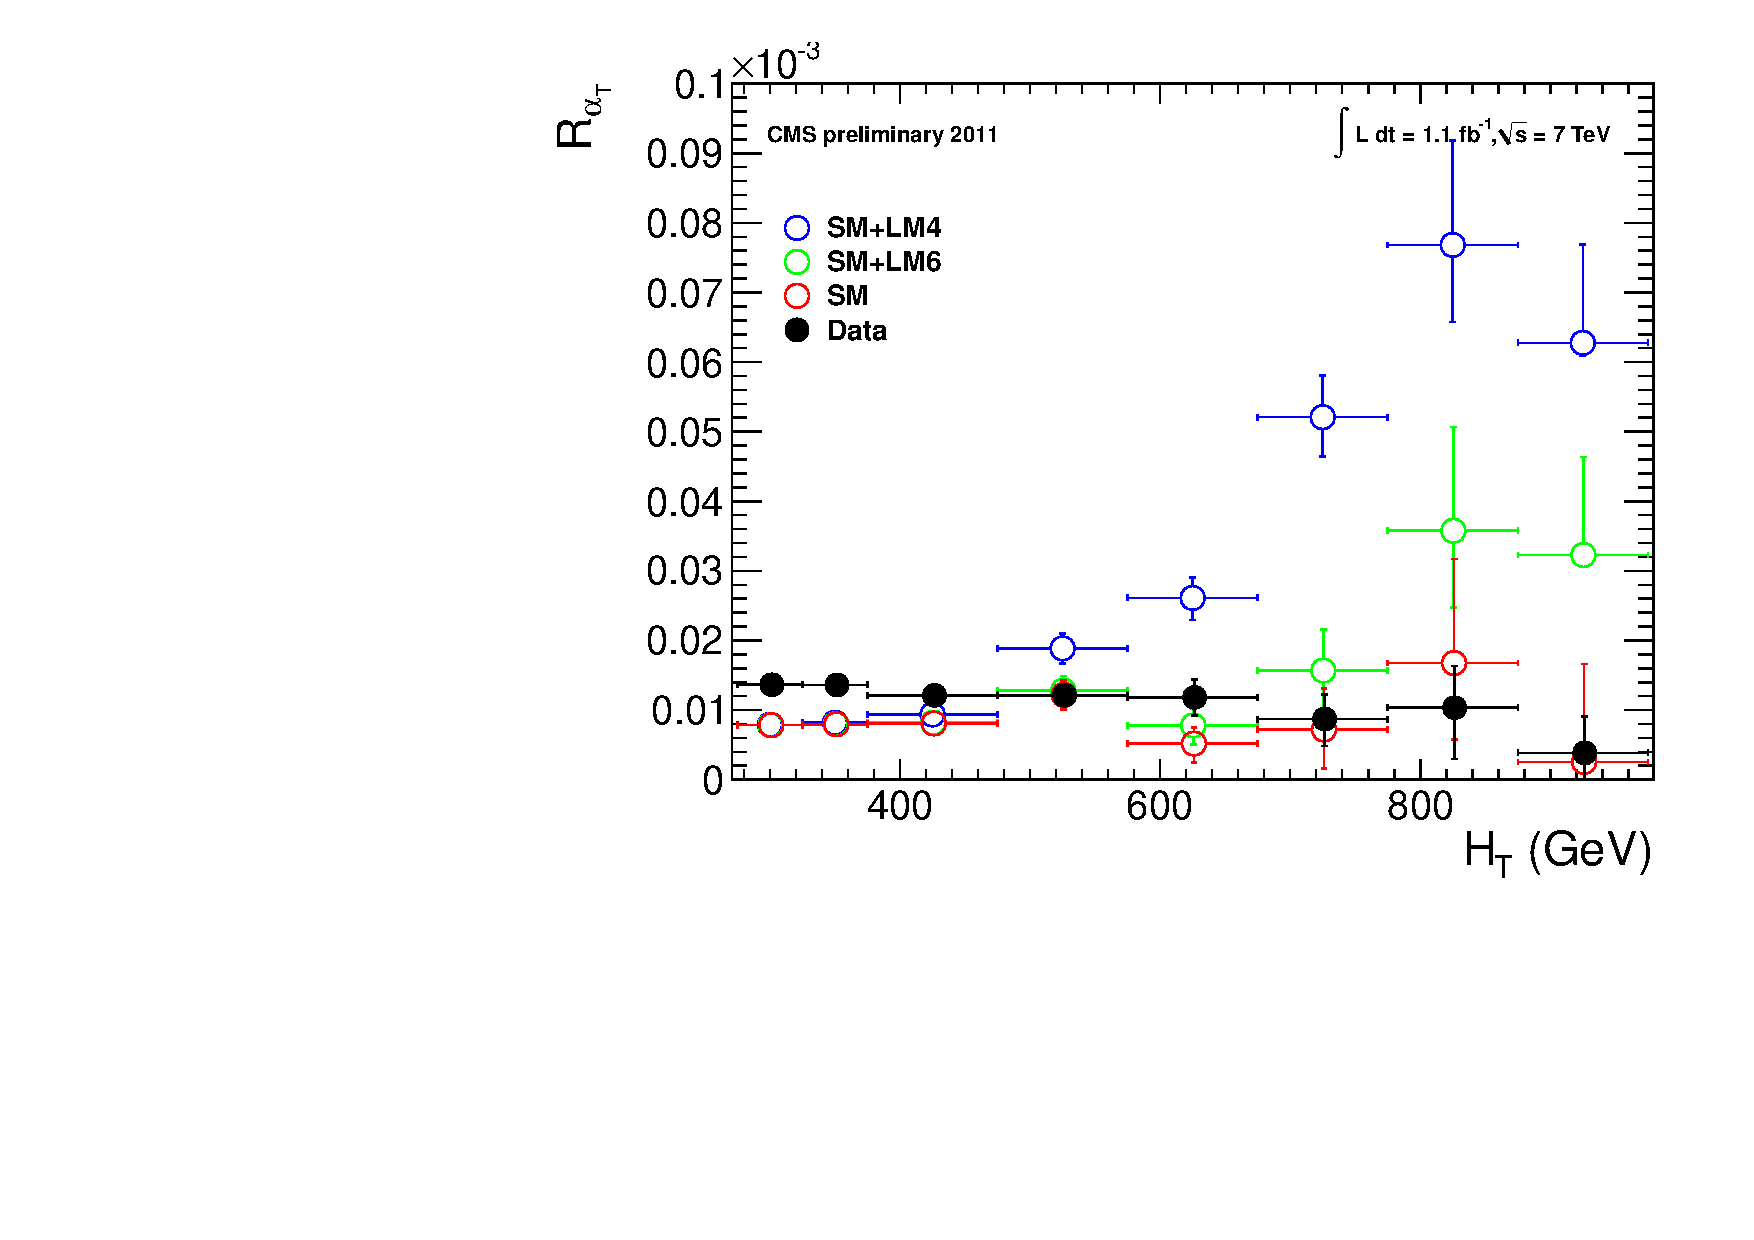
\includegraphics[width = 0.48\textwidth]{figures/Ratio_Multi2Incl_AlphaT55.pdf}
    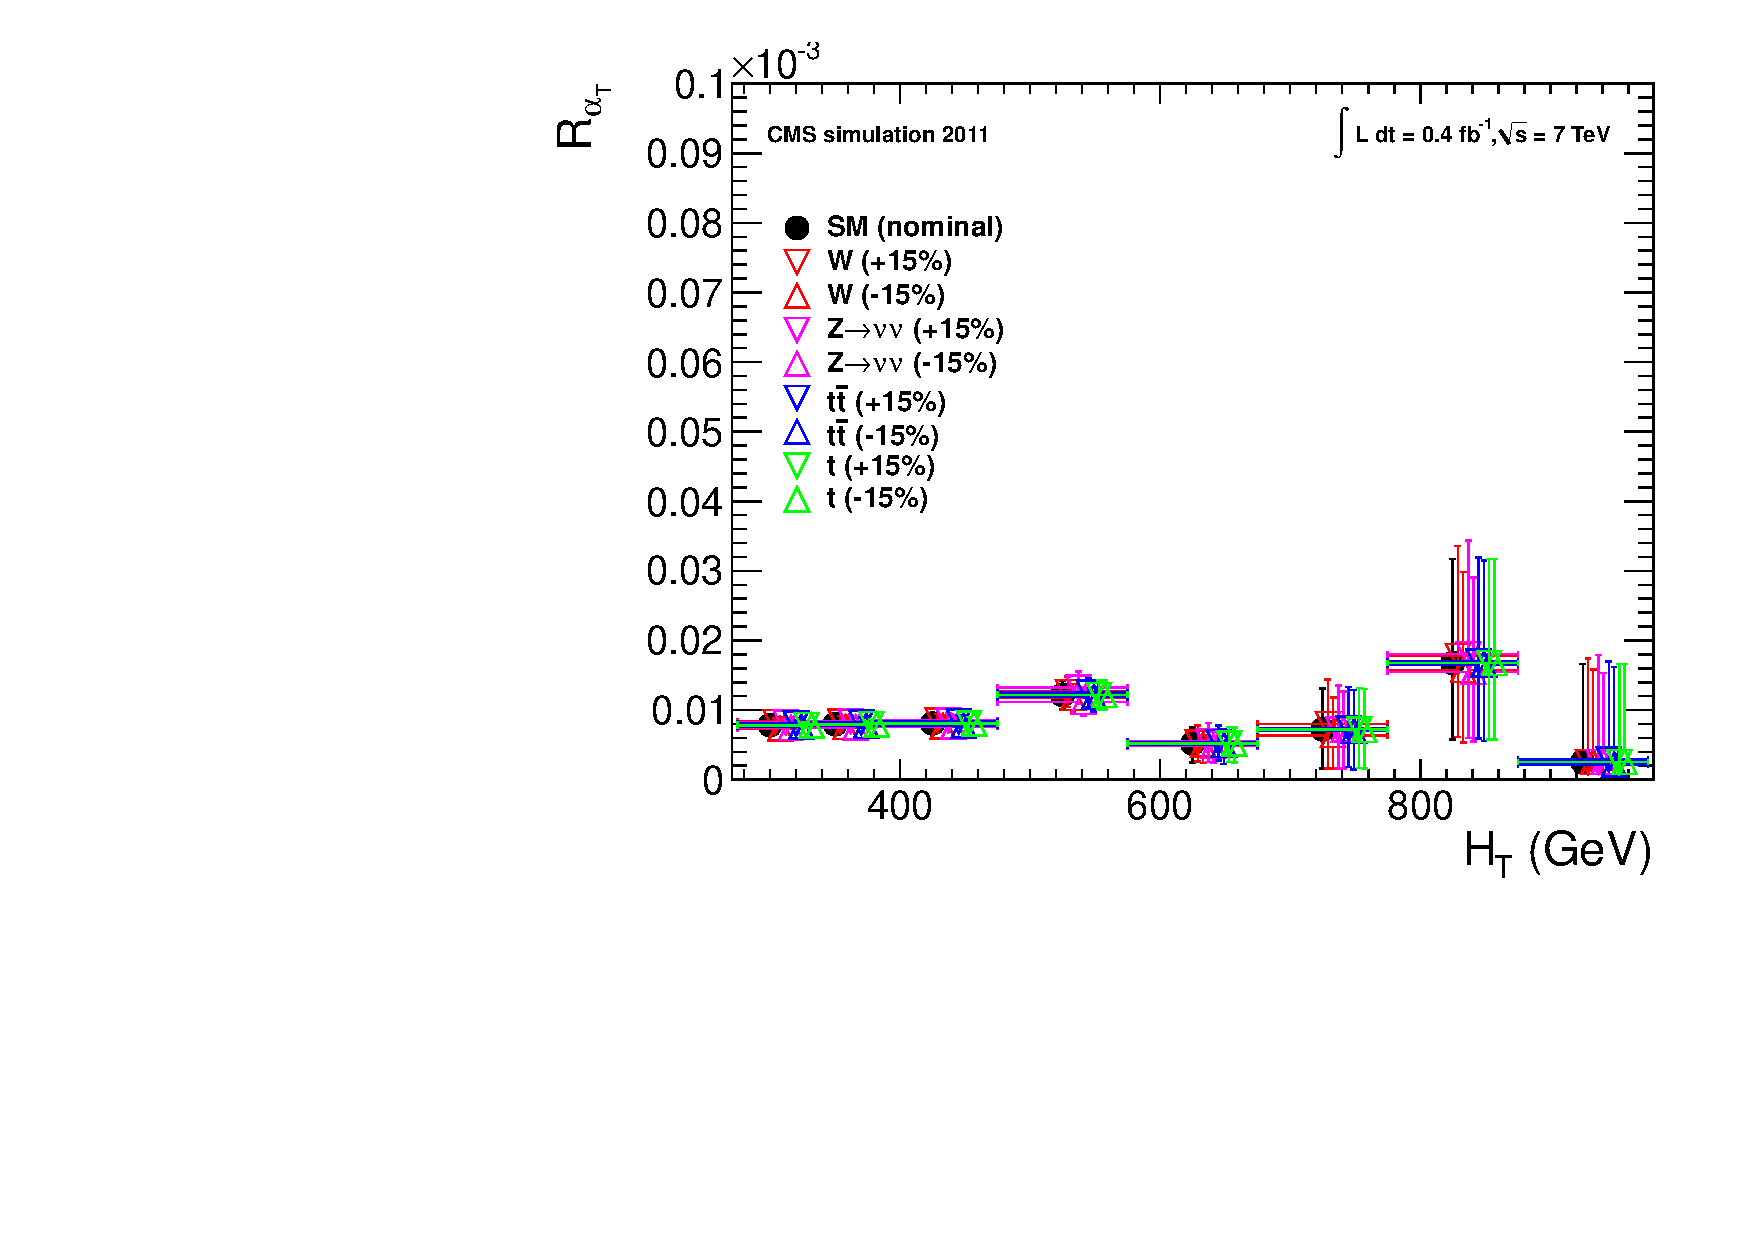
\includegraphics[width = 0.48\textwidth]{figures/Syst_Multi2Incl_AlphaT55.pdf}
    \caption{\label{fig:rat_vs_ht} (Left) The dependence of \RaT on
      \HT for events with N$_{\mathrm{jet}} \geq 2$. (Right) Dependence of \RaT on
      \HT when varying the effective cross-section of the four major
      EWK background components individually by $\pm$15\%. (Markers
      are artificially offset for clarity.)  }
  \end{center}
\end{figure}

\subsection{\scalht Dependence of \RaT  \label{sec:ht-scaling}}

The ratio $\RaT = N^{\alt > \theta}/N^{\alt < \theta}$ exhibits no
dependence on \scalht if $\theta$ is chosen such that the numerator of
the ratio in all \scalht bins is dominated by \ttbar, W +jets and
\znunu +jets events (referred to in the following as EWK) and there is
no significant contribution from events from QCD multi-jet
production~\cite{RA1Paper}. This is demonstrated in
Figure~\ref{fig:rat_vs_ht}, using MC simulations for the cut value
$\theta = 0.55$ over the range $275 < \scalht < 975 \gev$.

One important ingredient in the \RaT method is the scaling of the jet
\pt thresholds in the low \scalht bins to maintain jet multiplicities
and thus comparable event kinematics and topologies in the different
\scalht bins. This is especially important in the case of the \ttbar
background, which have on average a higher jet multiplicity then the
other EWK backgrounds.  If the jet \pt thresholds were not scaled
relative to \HT in the lowest \HT bins, \ttbar events would exhibit a
turn-on behaviour at low \HT before falling off exponentially like the
other SM backgrounds at high \HT.  Thus, in accordance with the 2010
analysis, the jet \pt thresholds are scaled only for the first two
\scalht bins, and remain fixed for all subsequent bins. The thresholds
are listed in Table~\ref{tab:results-HT}.  The ratio $\RaT = N^{\alt >
  \theta}/N^{\alt < \theta}$ exhibits no dependence on \scalht if
$\theta$ is chosen such that the numerator of the ratio in all \scalht
bins is dominated by \ttbar, W +jets and \znunu +jets events (referred
to in the following as EWK) and there is no significant contribution
from events from QCD multi-jet production~\cite{RA1Paper}. This is
demonstrated in Figure~\ref{fig:rat_vs_ht}, using MC simulations for
the cut value $\theta = 0.55$ over the range $275 < \scalht < 975
\gev$.

One important ingredient in the \RaT method is the scaling of the jet
\pt thresholds in the low \scalht bins to maintain jet multiplicities
and thus comparable event kinematics and topologies in the different
\scalht bins. This is especially important in the case of the \ttbar
background, which have on average a higher jet multiplicity then the
other EWK backgrounds.  If the jet \pt thresholds were not scaled
relative to \HT in the lowest \HT bins, \ttbar events would exhibit a
turn-on behaviour at low \HT before falling off exponentially like the
other SM backgrounds at high \HT.
Thus, in accordance with the 2010 analysis, the jet \pt thresholds are 
scaled only for the first two \scalht bins, and remain fixed for all
subsequent bins. The thresholds are listed in Table~\ref{tab:results-HT}.

Figure~\ref{fig:rat_vs_ht} (left) shows the dependence of \RaT on
\scalht, as measured in data and also obtained from MC simulations of
SM, and SM plus the SUSY benchmark points LM4 or LM6. The data (SM
expectations) are consistent with the flat hypothesis, with p-values
of 0.29 (0.50).  The SM+LM4 and SM+LM6 are not consistent with
constant $\RaT(\scalht)$, thus demonstrating that the presences of a
SUSY signal would result in a significant deviation from the
hypothesis of RaT being flat with \scalht .  As will be discussed in
more detail in Sec.~\ref{sec:statistics}, we also pursue an
alternative approach which allows for a small QCD contribution in the
low \HT regions. However, we have found no evidence in the 2011 data
that would invalidate the QCD free hypothesis, which in turn is
assumed to lead to \RaT being constant with \scalht .

Figure~\ref{fig:rat_vs_ht} (right) demonstrates the independence of
\RaT on \scalht, based on MC simulations, even when varying the
effective cross-section of the four major EWK background components
individually by as much as $\pm$15\%, which reflects our current
knowledge of the cross sections for these
backgrounds~\cite{top-xs,w-xs}. In each case, the behaviour is always
consistent with the flat hypothesis, with a p-value of at least
0.47. Studies with larger variations of $\pm$50\% also lead to
p-values that are consistent with the flat hypothesis. This is how the
assumption of flat behaviour is tested against the systematic
uncertainties associated with the cross-section measurements of the
different EWK backgrounds.

In 2010, a cut-based approach was used, in which an extrapolation from
a low-\scalht control region ($250 \GeV < \scalht < 350 \GeV$) into
the \scalht signal region ($\scalht > 350 \GeV$) was performed in
order to estimate the SM background. In the current analysis of the
2011 data, a shape analysis over the entire \HT $>$ 275 \GeV region is
carried out.


%{\bf Zoe}
\subsection{Estimation of Background from \ttbar and W + Jets Events using a Muon Control Sample \label{sec:mu}}

An estimate of the backgrounds from unidentified leptons and hadronic
tau decays originating from high-p$_{T}$ W bosons is obtained through
the use of a muon control sample. In this sample we explicitly select
W's decaying to a muon and a neutrino in the phase-space of the
signal. This is performed in the same \HT bins as for the hadronic
signal selection.

All cuts on jet-based quantities are consistent with those applied in
the hadronic search region.

In order to select W events we have the following additional cuts:
\begin{itemize}
\item  One isolated muon  with \PT $>$ 10 \gev and $|\eta| <$ 2.5.
\item $\mathrm{M_{T}} > 30$ GeV, where $\mathrm{M_{T}}$ is the transverse mass of the W candidate.
\item $\Delta$R(jet,muon) $> 0.5$
\item \mht/\scalht $>$ 0.4
\item No second isolated muon in the event. This reduces Z $\rightarrow \mu \mu$.
\end{itemize}

The number of events from W+jet events in the hadronic selection
$W_{data}^{had}$ can be estimated from the event yield, $W_{\rm
  data}^{\mu}$, of these type of events. This is done using the
expected relative ratio of those two types of events. The value of
this ratio is extracted from the MC, and thus the estimated number of
W events in the hadronic analysis is calculated by

\begin{displaymath}
W_{\rm data}^{\rm had} = W_{\rm data}^{\mu} \times \frac{W_{\rm MC}^{\rm had}}{W_{\rm MC}^{\mu}}.
\end{displaymath}

In the lowest two \HT bins, the value of $\frac{W_{\rm MC}^{\rm
    had}}{W_{MC}^{\mu}}$ is extracted separately. However, due to low
Monte Carlo statistics in the highest \HT bins, one value for the
ratio is used for $\HT > 375 \gev$.  The MC translation factor, which
is listed in Table~\ref{tab:results-W}, is expected to exhibit only a
weak dependence on HT Table~\ref{tab:results-W} shows the split of the
muon control sample numbers and the corresponding background
prediction in the different \scalht bins.  The errors quoted on the
predictions correspond to statistical errors and to an additional
systematic uncertainty of 30\%, as used in the previous
analysis~\cite{RA1Paper}.  There is good agreement between data and
MC, as shown both before (Figure \ref{fig:muonplots_beforeat}) and
after (Figure \ref{fig:muonplots_afterat}) the \alt cut.


\begin{table}[ht!]
\caption{\label{tab:results-W} Muon sample predictions with 1.1fb$^{-1}$. Errors quoted on predictions correspond to statistical errors and an additional conservative systematic uncertainty of 30\%, as used in the previous analysis.}
\centering
%\footnotesize
\scriptsize
\begin{tabular}{ c|c|c|c|c }
\hline
\scalht Bin (GeV)       & 275--325                       & 325--375                       & 375--475                       & 475--575                       \\ [0.5ex]
\hline
MC W + $\ttNew$         & 463.0 $\pm$ 16.0$_{\rm stat}$      & 171.2 $\pm$  9.5$_{\rm stat}$      & 116.3 $\pm$  8.3$_{\rm stat}$      & 43.7 $\pm$  5.1$_{\rm stat}$       \\ 
MC $\mu +$~jets         & 407.5 $\pm$ 14.5$_{\rm stat}$      & 179.1 $\pm$  9.6$_{\rm stat}$      & 131.6 $\pm$  8.8$_{\rm stat}$      & 48.7 $\pm$  5.5$_{\rm stat}$       \\ 
MC Ratio                & 1.14                           & 0.96                           & 0.90                           & 0.90                           \\ 
Data $\mu +$~jets       & 389                          & 156                          & 113                         &  39                          \\ 
W + $\ttNew$ Prediction & 442.0 $\pm$  22.4$_{\rm stat}$  $\pm$
132.6$_{\rm syst}$ & 149.1 $\pm$  11.9$_{\rm stat}$  $\pm$  44.7$_{\rm
  syst}$ & 101.9 $\pm$   9.6$_{\rm stat}$  $\pm$  30.6$_{syst}$ & 35.2 $\pm$   5.6$_{\rm stat}$  $\pm$  10.6$_{\rm syst}$ \\ 
\hline
\scalht Bin (GeV)       & 575--675                       & 675--775                       & 775--875                       & 875--$\infty$                  \\ [0.5ex]
\hline
MC W + $\ttNew$         & 17.5 $\pm$  3.2$_{\rm stat}$       &  5.1 $\pm$  1.8$_{\rm stat}$       &  1.1 $\pm$  0.7$_{\rm stat}$       &  1.8 $\pm$  1.0$_{\rm stat}$       \\ 
MC $\mu +$~jets         & 13.3 $\pm$  2.9$_{\rm stat}$       &  8.0 $\pm$  2.3$_{\rm stat}$       &  3.2 $\pm$  1.4$_{\rm stat}$       &  0.9 $\pm$  0.7$_{\rm stat}$       \\ 
MC Ratio                & 0.90                           & 0.90                           & 0.90                           & 0.90                           \\ 
Data $\mu +$~jets       &  17                          &   5                          &   0                          &   0                          \\ 
W + $\ttNew$ Prediction &  15.3 $\pm$   3.7$_{\rm stat}$  $\pm$
4.6$_{\rm syst}$ &   4.5 $\pm$   2.0$_{\rm stat}$  $\pm$   1.4$_{\rm syst}$ &   0.0 $\pm$   1.0$_{\rm stat}$     &   0.0 $\pm$   1.0$_{\rm stat}$     \\ 
\hline
\end{tabular}
\end{table}

\begin{figure}[!h]
\begin{center}
\subfigure[\label{fig:muon_beforeat_at}]{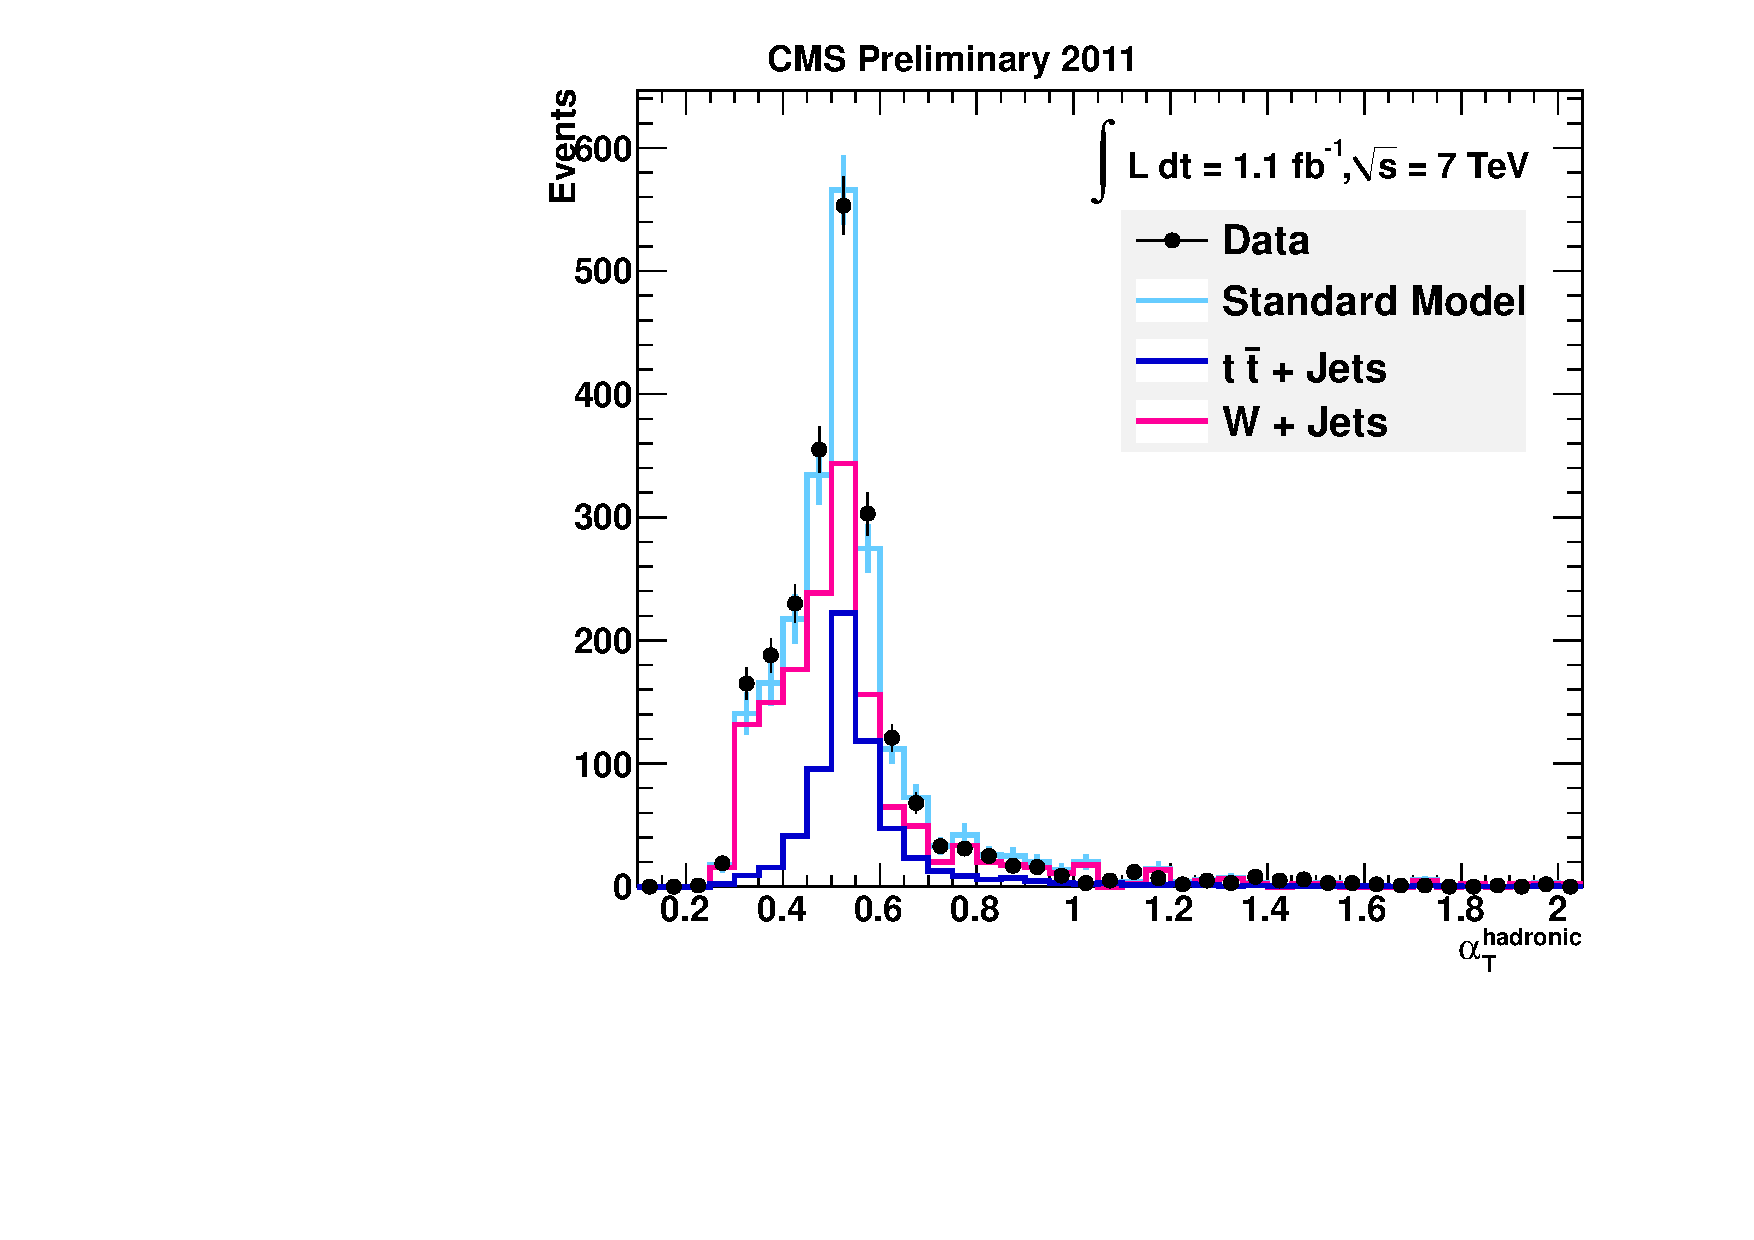
\includegraphics[width=0.45\textwidth, angle=0]{figures/muon_plots/spring11NoLogYaT_HMuonControl_beforeaT.pdf}}
\subfigure[\label{fig:muon_beforeat_ht}]{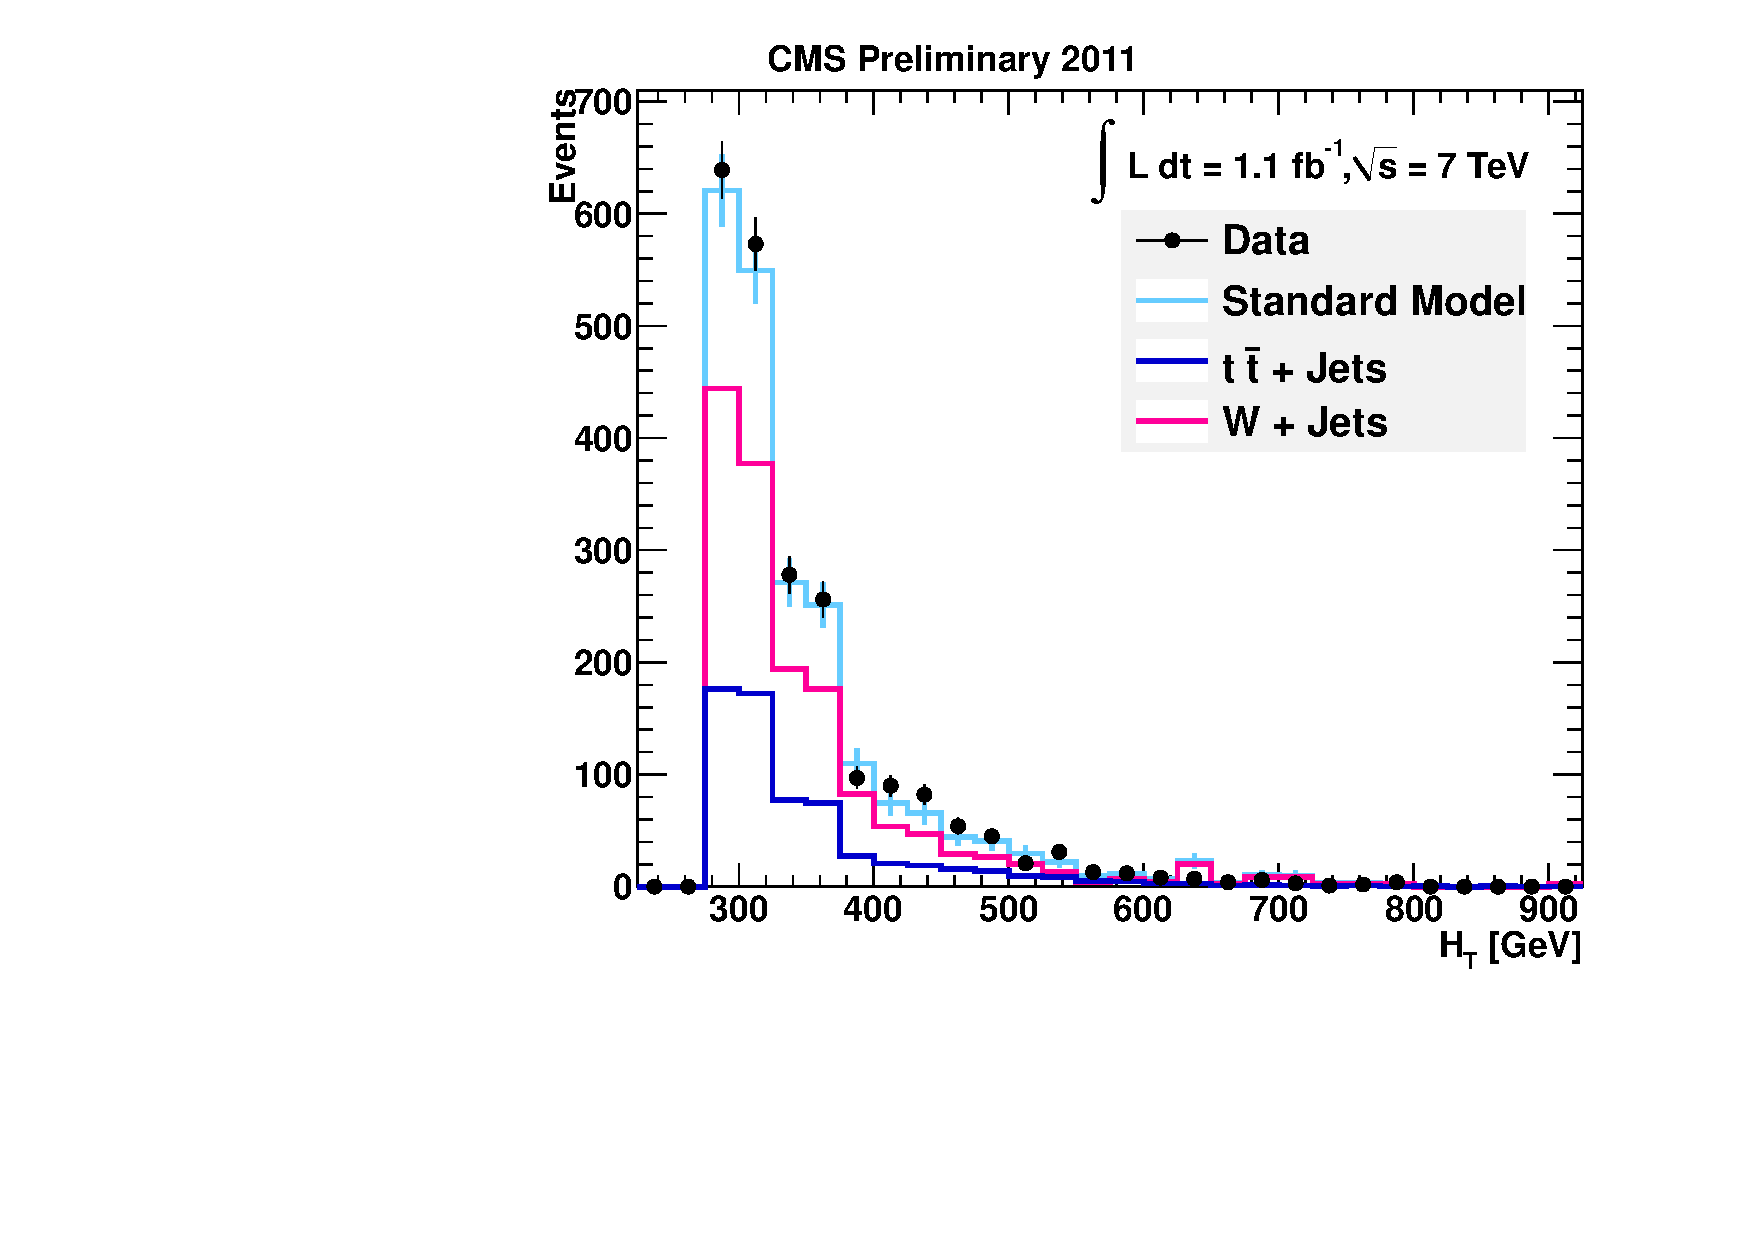
\includegraphics[width=0.45\textwidth, angle=0]{figures/muon_plots/spring11NoLogYHTMuonControl_beforeaT.pdf}}
\newline

\caption{\label{fig:muonplots_beforeat} Data - Monte Carlo comparisons
  for the muon control selection before the $\alpha_{T} > 0.55$ cut is
  applied, shown for (a) $\alpha_{T}$ and (b) $H_{T}$.%, (c) Muon  Combined Isolation and (d) $M_{T}$.
 A cut of $\mathrm{HT >}$375 GeV has been applied, to select the
 region of fixed jet thresholds.}
\label{fig:kin}
\end{center}
\end{figure}

\begin{figure}[!h]
\begin{center}
%\subfigure[\label{fig:muon_afterat_at}]{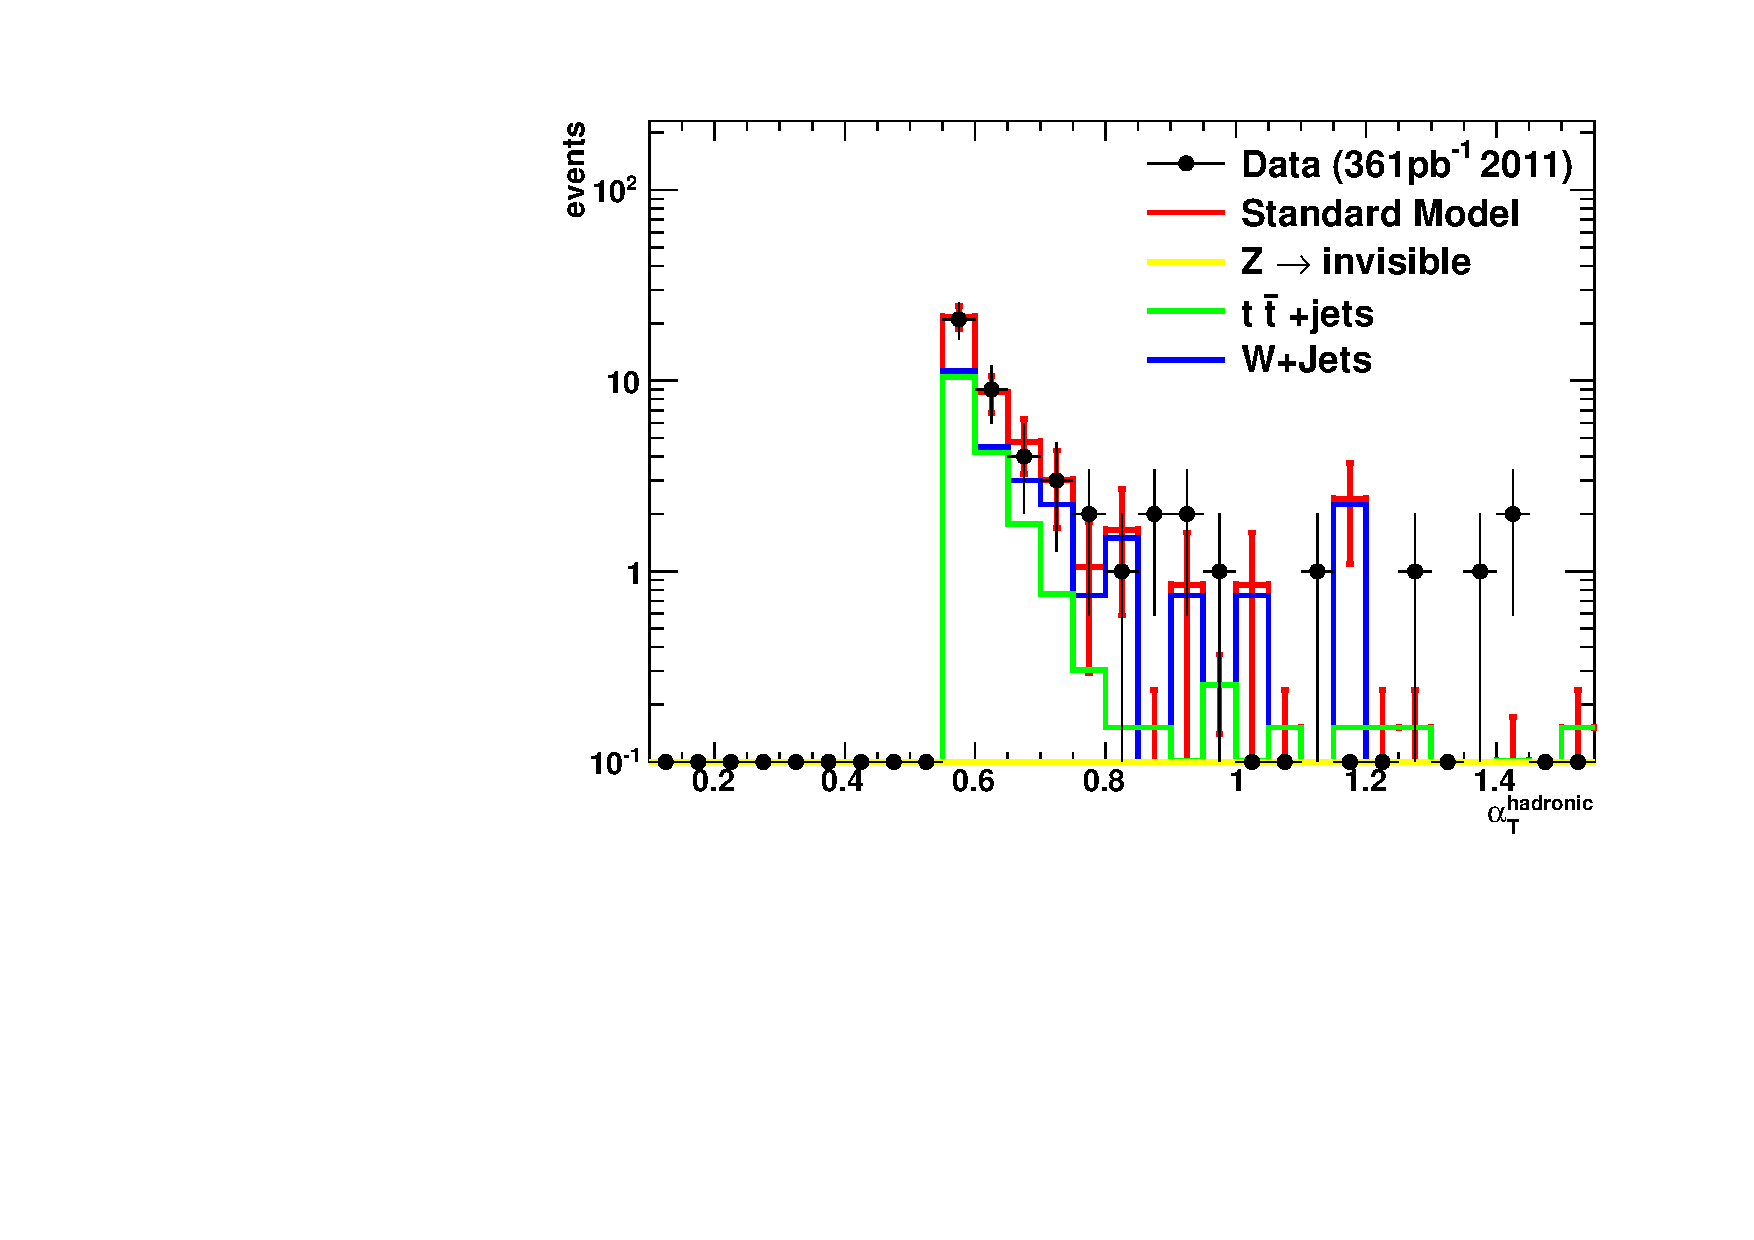
\includegraphics[width=0.45\textwidth, angle=0]{figures/MuonControl_afteraT_aT.pdf}}
\subfigure[\label{fig:muon_afterat_ht}]{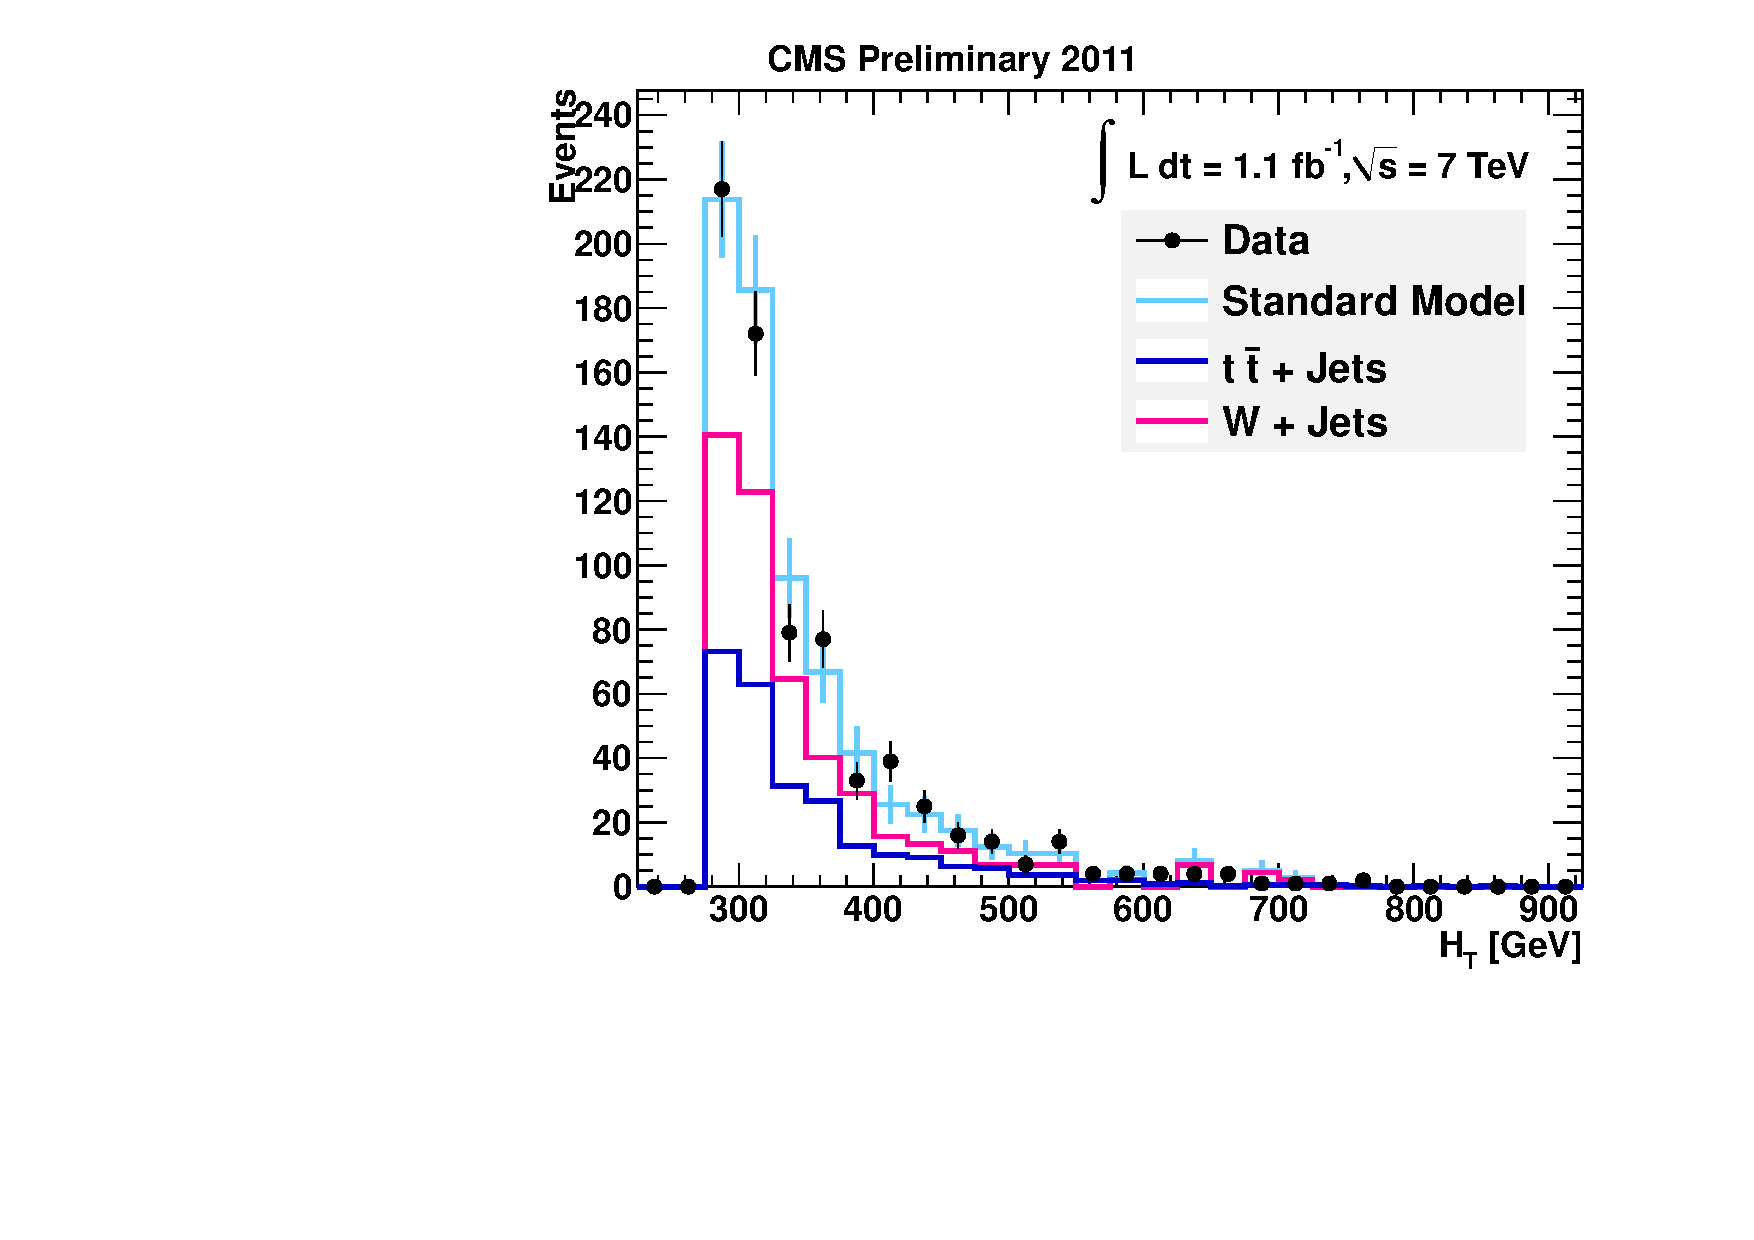
\includegraphics[width=0.45\textwidth, angle=0]{figures/muon_plots/spring11NoLogYHTMuonControl_afteraT.pdf}}
%\newline
%\subfigure[\label{fig:muon_afterat_MuIso}]{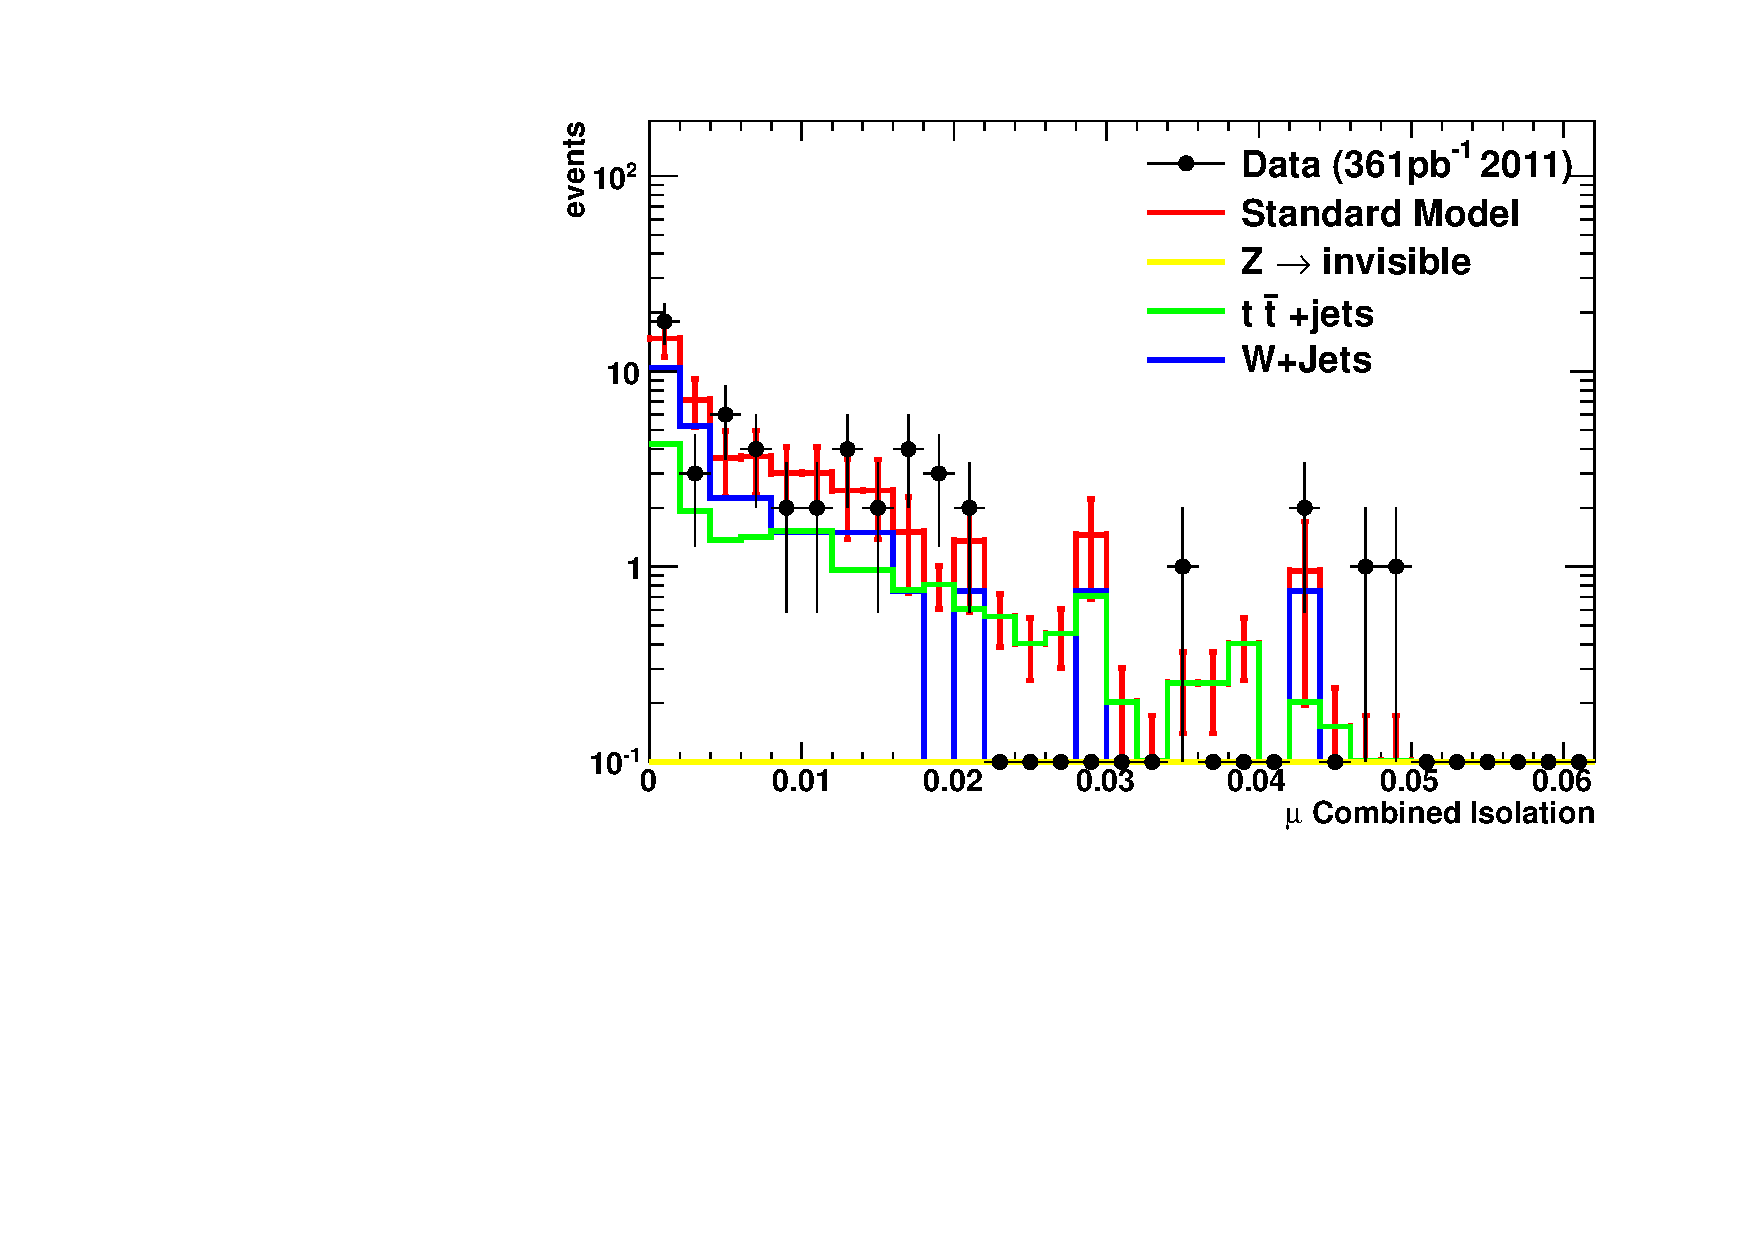
\includegraphics[width=0.45\textwidth, angle=0]{figures/MuonControl_afteraT_MuonCombIso.pdf}}
\subfigure[\label{fig:muon_afterat_mt}]{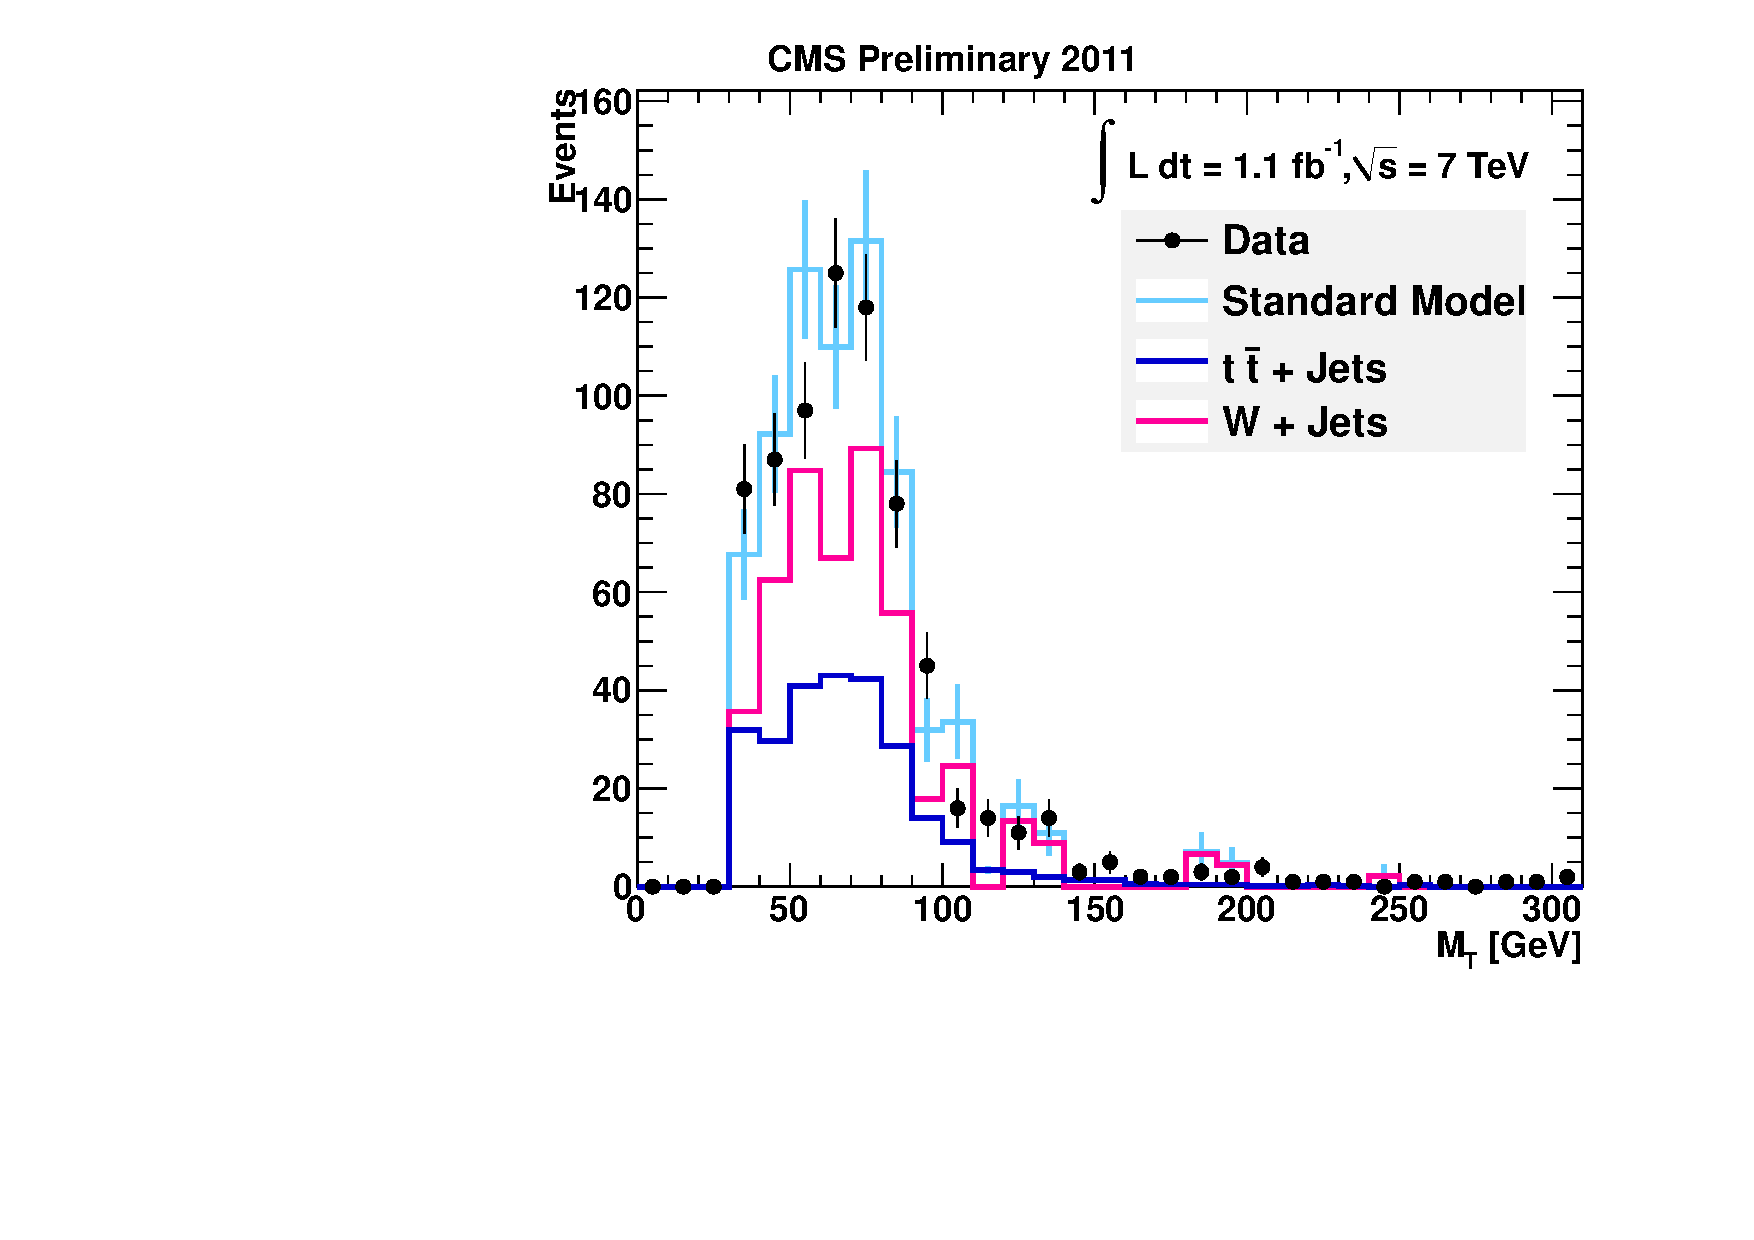
\includegraphics[width=0.45\textwidth, angle=0]{figures/muon_plots/spring11NoLogYMTMuonControl_afteraT.pdf}}

\caption{\label{fig:muonplots_afterat} Data - Monte Carlo comparisons
  for the muon control selection after the $\alpha_{T} > 0.55$ cut is
  applied, shown for (a) \scalht and (b) $M_T$.%, (c) Muon  Combined Isolation and (d) $M_{T}$.
 A cut of $\mathrm{HT >}$375 GeV has been applied, to select the
 region of fixed jet thresholds.}
\label{fig:kin}
\end{center}
\end{figure}


\subsection{Estimation of Background from \znunu + Jets from Photon + Jets Events\label{sec:photon}}

\znunu\ +jet events form an irreducible background.  An estimate of
this background can be obtained from the $\gamma$ + jets process,
which has a larger cross section but kinematic properties similar to
those of \znunu\ events when the photon is ignored (see
e.g. ~\cite{cms-pas-sus-08005} and ~\cite{Bern:2011pa}).  The $\gamma$
+ jet sample is selected by requiring photons, i.e. localized
electromagnetic depositions satisfying tight isolation
criteria %\cite{photon_id}
, with $\pt$ greater than 100 \gev, $|\eta|$ less than 1.45 and
$\Delta R (\gamma, {\rm jet}) >1$. Ignoring the photon, the same
hadronic final state selection as in the signal selection is applied.

\begin{figure}[!h]
\begin{center}
\subfigure[\label{fig:photon_alphaT}]{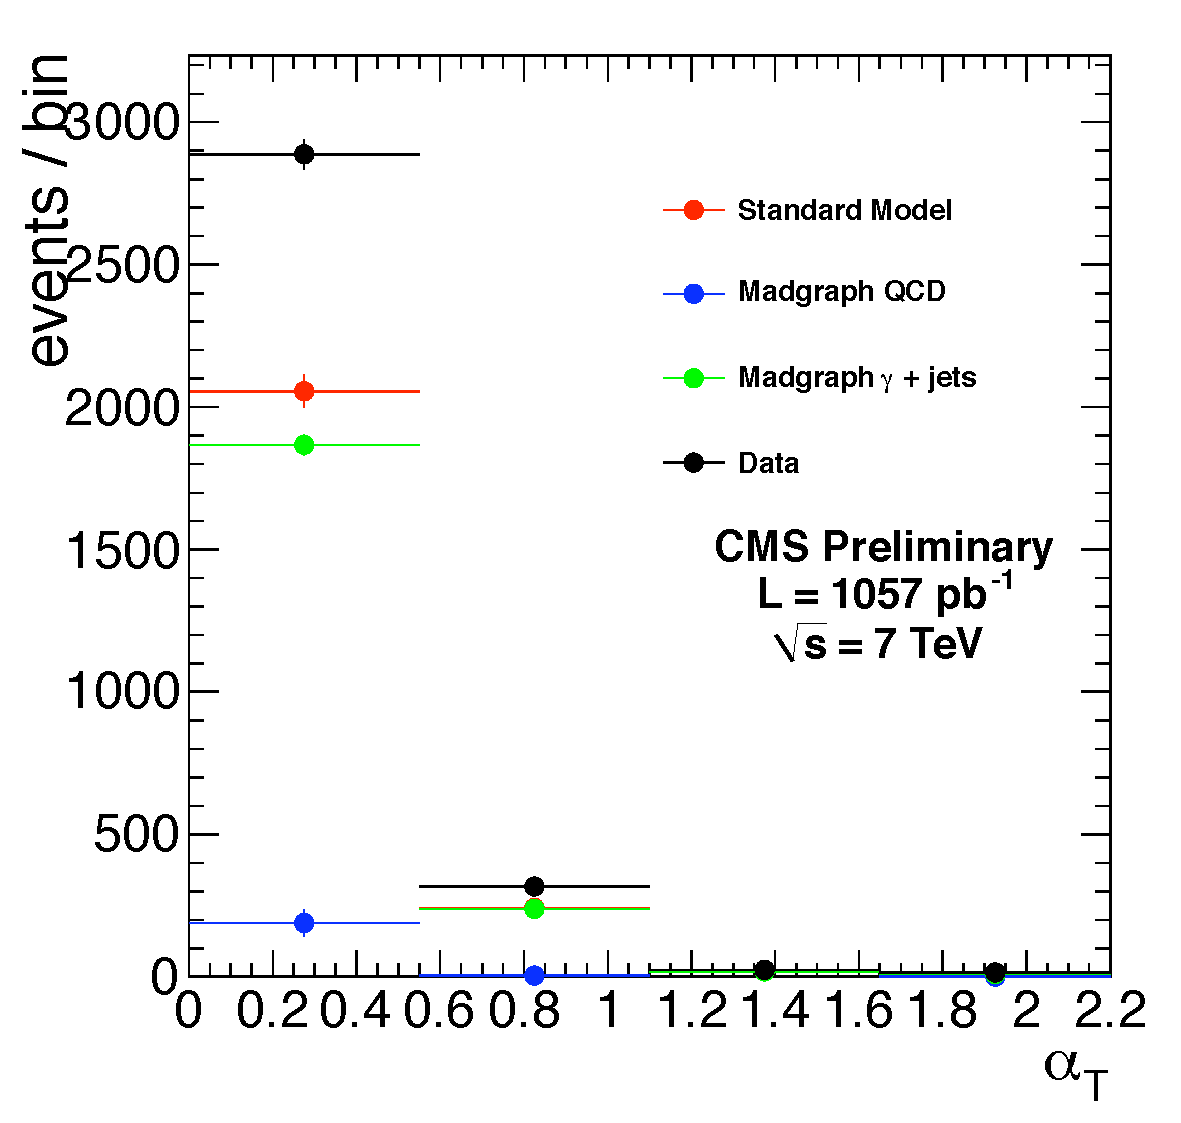
\includegraphics[width=0.45\textwidth, angle=0]{figures/photon_plots/375___xcak5JetAlphaTFewBinsPat.pdf}}
\subfigure[\label{fig:photon_nJets}] {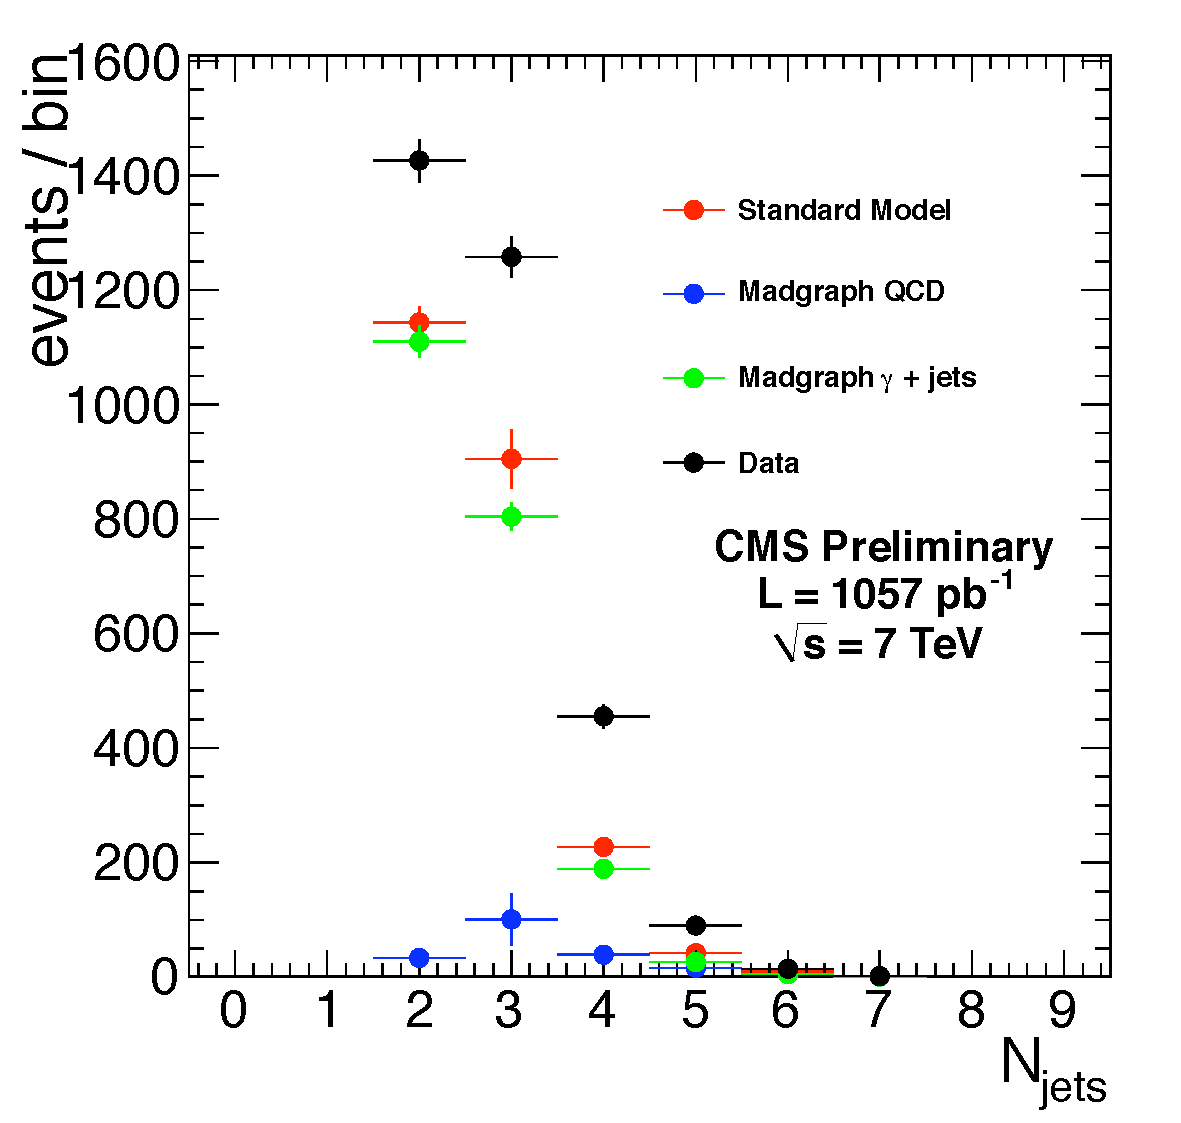
\includegraphics[width=0.45\textwidth, angle=0]{figures/photon_plots/375___xcak5JetIndicesPat.pdf}}
\caption{\label{fig:photon_plots} Data-MC comparisons for the photon control sample.  $\scalht > 375$~GeV and $\mht/\scalht>0.4$ are required.   Left: the distribution of $\alpha_{T}$.  Right: the distribution of the number of jets.}
\end{center}
\end{figure}

Table~\ref{tab:results-PHOTON} shows the observed counts in the photon
control sample and the corresponding background predictions.  As in
~\cite{RA1Paper}, we use a 40\% total systematic uncertainty on the
method.  Figure~\ref{fig:photon_plots} shows the \alt and jets
multiplicity distributions for the selected photon control sample.


\begin{table}[ht!]
\caption{Photon Sample Predictions 1.1fb$^{-1}$}
\label{tab:results-PHOTON}
\centering
%\footnotesize
\scriptsize
\begin{tabular}{ c|c|c|c|c }

\hline
\scalht Bin (GeV)       & 275--325                       & 325--375                       & 375--475                       & 475--575                       \\ [0.5ex]
\hline
MC $\znunu$             & 212.6 $\pm$ 20.4$_{\rm stat}$      & 92.0 $\pm$ 20.4$_{\rm stat}$       & 61.3 $\pm$ 20.4$_{\rm stat}$       & 42.9 $\pm$ 10.2$_{\rm stat}$       \\ 
MC $\gamma +$~jets      & 613.1 $\pm$ 20.4$_{\rm stat}$      & 265.7 $\pm$ 10.2$_{\rm stat}$      & 168.6 $\pm$ 10.2$_{\rm stat}$      & 55.2 $\pm$  8.2$_{\rm stat}$       \\ 
MC Ratio                & 0.35                           & 0.35                           & 0.44                           & 0.44                           \\ 
Data $\gamma +$~jets    & 867.5                          & 313.7                          & 214.6                          &  68.5                          \\ 
Sample Purity           & 0.92                           & 0.97                           & 0.99                           & 0.99                           \\ 
$\znunu$ Prediction     & 276.8 $\pm$   9.5$_{\rm stat}$  $\pm$ 110.7$_{syst}$ & 105.3 $\pm$   6.0$_{\rm stat}$  $\pm$  42.1$_{syst}$ &  93.5 $\pm$   6.4$_{\rm stat}$  $\pm$  37.4$_{syst}$ &  29.8 $\pm$   3.6$_{\rm stat}$  $\pm$  11.9$_{syst}$ \\ 

\hline
\scalht Bin (GeV)       & 575--675                       & 675--775                       & 775--875                       & 875--$\infty$                  \\ [0.5ex]
\hline
MC $\znunu$             &  5.1 $\pm$  5.1$_{\rm stat}$       &  0.0 $\pm$  3.1$_{\rm stat}$       &  3.1 $\pm$  3.1$_{\rm stat}$       &  0.0 $\pm$  3.1$_{\rm stat}$       \\ 
MC $\gamma +$~jets      & 23.5 $\pm$  5.1$_{\rm stat}$       &  3.1 $\pm$  2.0$_{\rm stat}$       &  3.1 $\pm$  2.0$_{\rm stat}$       &  2.0 $\pm$  1.0$_{\rm stat}$       \\ 
MC Ratio                & 0.44                           & 0.44                           & 0.44                           & 0.44                           \\ 
Data $\gamma +$~jets    &  24.5                          &  12.3                          &   4.1                          &   4.1                          \\ 
Sample Purity           & 0.99                           & 0.99                           & 0.99                           & 0.99                           \\ 
$\znunu$ Prediction     &  10.7 $\pm$   2.2$_{\rm stat}$  $\pm$   4.3$_{syst}$ &   5.3 $\pm$   1.5$_{\rm stat}$  $\pm$   2.1$_{syst}$ &   1.8 $\pm$   0.9$_{\rm stat}$  $\pm$   0.7$_{syst}$ &   1.8 $\pm$   0.9$_{\rm stat}$  $\pm$   0.7$_{syst}$ \\ 

\hline
\end{tabular}
\end{table}


\subsection{Background Cross-Check: Estimation of \wmunu + Jets Events
from Photon + Jets Events}

To verify that our background estimation method for \znunu~events is
performing as expected, and that the assigned systematic uncertainties
are adequate, we use the photon + jets sample to predict the number of
\wmunu~events, which is kinematically similar to the process \znunu +
jets. To reject events originating from \ttbar production, and to
obtain a pure W + jets sample, the number of jets is limited to two.
The number of W events can then be obtained as follows:

\begin{displaymath}
N_{\rm data}^{W} = N_{\rm data}^{\rm phot} \times \frac{N_{\rm MC}^{W}}{N_{\rm MC}^{\rm phot}}.
\end{displaymath}

The factor $\frac{N_{\rm MC}^{W}}{N_{\rm MC}^{\rm phot}}$, which
corrects for selection efficiencies and acceptance, is taken from MC
simulation.  Within the statistical precision of the MC sample, it is
found to be approximately independent of \HT.  We thus use a constant
factor of $0.42\pm 0.04$.  The results are summarized in
Table~\ref{tab:results-photW} and the predicted number of muon events
is in good agreement with the observed number within the assigned
systematic uncertainties.

\begin{table}[ht!]
\caption{Predictions of W + two jets events using the photon sample 1.1fb$^{-1}$.}
\label{tab:results-photW}
\centering
\footnotesize
\begin{tabular}{ c|c|c|c|c }
\hline
\HT & $N_{\rm data}^{\rm phot}$ & $N_{\rm MC}^W/N_{\rm MC}^{\rm phot}$ & $N^{W}_{\rm pred W}$ &$N^{W}_{\rm obs}$ \\
\hline
%275     &  336   &    0.42 $\pm$ 0.07  &  141.2 $\pm$ 7.7 (stat)  $\pm$ 22.1 (MC stat) $\pm$  56.5 (syst)&  128\\
%325     &  127  &     0.44 $\pm$ 0.06 &  55.7 $\pm$  4.9 (stat) $\pm$  7.7 (MC stat)  $\pm$  22.3 (syst)&    37\\
%375     &  136    &   0.66 $\pm$ 0.09 &  90.3 $\pm$  7.7 (stat) $\pm$  12.7 (MC stat)  $\pm$  36.1 (syst)&    50\\

275    &    336  &     0.42 $\pm 0.04_{\rm MCstat}$ & 141.8 $\pm 7.7_{\rm stat} \pm 14.6_{\rm MCstat} \pm  56.7_{\rm syst}$&  128\\
325    &    127  &     0.42 $\pm 0.04_{\rm MCstat}$ &   53.6 $\pm 4.8_{\rm stat} \pm  5.5_{\rm MCstat} \pm  21.4_{\rm syst}$&    37\\
375    &      96  &     0.42 $\pm 0.04_{\rm MCstat}$ &   40.5 $\pm 4.1_{\rm stat} \pm  4.2_{\rm MCstat} \pm  16.2_{\rm syst}$ &   36\\
475    &      27  &     0.42 $\pm 0.04_{\rm MCstat}$ &   11.4 $\pm 2.2_{\rm stat} \pm  1.2_{\rm MCstat} \pm  4.6_{\rm syst}$&   12\\
575    &       13 &     0.42 $\pm 0.04_{\rm MCstat}$ &     5.5 $\pm 1.5_{\rm stat} \pm  0.6_{\rm MCstat} \pm   2.2_{\rm syst}$&    2 \\

\hline

\end{tabular}
\end{table}
